\documentclass[final,review]{siamart}
%\documentclass[a4paper,10pt,reqno]{amsart}
%\usepackage[utf8]{inputenc}
\usepackage{amsmath,amsfonts}
%\usepackage{amsmath,amssymb,amsthm,dsfont}
%\usepackage{dsfont,amssymb}
%\usepackage[top = 3cm, bottom = 3cm, left = 3.0cm, right = 3.0cm]{geometry}
%\usepackage[notcite,notref]{showkeys}
%\usepackage{mathtools}
\usepackage{graphicx}
\usepackage{multirow}
\usepackage{pgfplots}
%\usepackage{tikz}
\pgfplotsset{compat=newest}
\usepackage{caption}
\usepackage{subcaption}
\usepackage{float}
\usepackage{cases}
%MACROs



\providecommand{\norm}[1]{\lVert#1\rVert}
\def\be{\begin{equation}}
\def\ee{\end{equation}}

\def\beal{\begin{equation}\begin{aligned}}
\def\eeal{\end{aligned}\end{equation}}

\def\bea{\begin{equation*}\begin{aligned}}
\def\eea{\end{aligned}\end{equation*}}

\def\bealn{\begin{equation}\left\{\begin{aligned}}
\def\eealn{\end{aligned}\right.\end{equation}}

\def\bean{\begin{equation*}\left\{\begin{aligned}}
\def\eean{\end{aligned}\right.\end{equation*}}

\def\besn{\begin{subequations}\begin{numcases}{}}
\def\eesn{\end{numcases}\end{subequations}}

\providecommand{\abs}[1]{\lvert#1\rvert}
\providecommand{\megaabs}[1]{\left\lvert#1\right\rvert}
\def\lspace{L^2(\Omega,L^2(I))}
%\def\M{\mathcal{M}_I}
\def\M{\mathcal{M}(\Omega_c, L^{2}(I))}
\def\Mc{\mathcal{M}(\Omega_{c}, L^{2}(I))}
\def\C{\mathcal{C}(\Omega_c, L^{2}(I))}
\def\R{\mathbb{R}}
\def\N{\mathbb{N}}
\def\B{\mathcal{B}}
\def\Hm1{L^2(I,H^{-1}(\Omega))}
\def\KdVB{KdVB }
\def\KdV{KdV }
\newcommand{\BigO}[1]{\ensuremath{\operatorname{O}\bigl(#1\bigr)}}
\def\bem{\begin{multline}}
\def\endmult {\end{multline}}
\def\rg{\varepsilon}
\def\SO{S_{obs}}
\newtheorem{remark}[theorem]{Remark}

% \newtheoremstyle{slplain}% name
%   {0.5\baselineskip\@plus.2\baselineskip\@minus.2\baselineskip}% Space above
%   {0.5\baselineskip\@plus.2\baselineskip\@minus.2\baselineskip}% Space below
%   {\itshape}% Body font
%   {}%Indent amount (empty = no indent, \parindent = para indent)
%   {\bfseries}%  Thm head font
%   {.}%       Punctuation after thm head
%   { }%      Space after thm head: " " = normal interword space;
%         %       \newline = linebreak
%   {}%       Thm head spec
%
%
% \theoremstyle{slplain}

%\newtheorem{thm}{Theorem}[section]
%\newtheorem{prop}[thm]{Proposition}
%\newtheorem{lem}[thm]{Lemma}
%\newtheorem{cor}[thm]{Corollary}
%\newtheorem{Def}[thm]{Definition}
%\newtheorem{rmk}[thm]{Remark}
%\newtheorem{as}[thm]{Assumption}

% ===================================================================
% Color
% ===================================================================

%\usepackage{xcolor}
%\definecolor{myorange}{rgb}{0.9568,0.4941,0.1961}
%\definecolor{myred}{rgb}{0.9098,0.1294,0.2078}
%\definecolor{myblue}{rgb}{0.0352,0.4981,0.6509}
%\definecolor{myhyperblue}{rgb}{0.1607,0.3922,0.9}
%\definecolor{mygreen}{rgb}{0.2235,0.6353,0.2588}
%\definecolor{mygrey}{rgb}{0.3,0.3,0.3}

%====================================================================
% HyperRef
%====================================================================
%\usepackage{hyperref}
%\hypersetup{
%pdfborder=0 0 0,
%colorlinks=true,
%linkcolor=mygrey,
%citecolor=myhyperblue
%}

\DeclareMathOperator{\shrink}{shrink}


\renewcommand{\thetheorem}{\thesection.\arabic{theorem}}
\renewcommand{\theequation}{\thesection.\arabic{equation}}
\renewcommand{\thefigure}{\thesection.\arabic{figure}}
%opening

%Submitted, 09.05.2015

\begin{document}

\title{Sparse optimal control of the Korteweg-de Vries-Burgers equation on a bounded domain}

\author{Anne-Celine Boulanger\footnotemark[3]\ \footnotemark[5]
\and Philip Trautmann\footnotemark[2]\ \footnotemark[5]}


\pagestyle{myheadings}
\thispagestyle{plain}
\markboth{A.-C. BOULANGER, P. TRAUTMANN}{SPARSE CONTROLS FOR THE KdV EQUATION}

\maketitle

\renewcommand{\thefootnote}{\fnsymbol{footnote}}

\footnotetext[2]{Institute for Mathematics and Scientific Computing, University of Graz,
  Heinrichstrasse 36, A-8010 Graz, Austria, (philip.trautmann@uni-graz.at).}

\footnotetext[3]{Chair of Optimal Control, Technische Universit\"at M\"unchen,
  Boltzmannstra{\ss}e 3, 85748 Garching bei M\"unchen, Germany
  (boulanger@ma.tum.de).}

\footnotetext[5]{Both authors gratefully acknowledges support from
the International Research Training Group IGDK1754, funded by the DFG and FWF.}


\renewcommand{\thefootnote}{\arabic{footnote}}




\maketitle

\slugger{sicon}{xxxx}{xx}{x}{x--x}%slugger should be set to mms, siap, sicomp, sicon, sidma, sima, simax, sinum, siopt, sisc, or sirev

\begin{abstract}
In this work we consider measure-valued optimal control problems involving the KdV-Burgers equation as state equation. These optimal control problems are motivated by an inverse problem and a control problem involving the flow of water in a channel over topography. Well-posedness of the optimal control problem is established which involves the investigation of the KdV-Burgers equation for irregular source terms. Moreover optimality conditions for the control problem are derived. Efficient numerical schemes based on spectral methods are proposed for the state and adjoint equation, as well as adequate optimization methods. The work is illustrated by several numerical examples.
\end{abstract}

\begin{keywords}Sparse optimal control, Korteweg-de Vries equation, Inverse problem, Spectral methods\end{keywords}

\begin{AMS}35Q93,49J20, 65M70, 74J30\end{AMS}

%!TEX root = kdv.tex

\section{Introduction}

The Korteweg-de Vries equation first appeared in 1895 in the context of water waves \cite{korteweg1895xli}. It was designed to model the evolution of long water waves in a channel of rectangular cross section when the effects of nonlinearity and dispersion balance. This phenomenon gives rise to the so-called solition, a solitary wave traveling at constant speed without losing its shape. This equation has been theoretically widely studided: much work has been devoted to the derivation of both equations from Euler equations \cite{shen1992forced,constantin2008,su2003korteweg}, but also to the proof of their well-posedness in various contexts \cite{miura1976korteweg,kenig1993,bourgain1997periodic} - periodic domain, on the real line, bounded domain -, to their controllability \cite{rosier1997exact,glass2008some,coron2003exact,chapouly2009global}. 
Because many applications were investigated, and in particular, numerous works in environmental sciences but also life sciences - see \cite{dauxois2006physics,whitham2011linear,Crepeau2007594,yomosa1987} and the references therein, lots of numerical methods have been developped to solve it efficiently \cite{trefethen2000spectral,shen2003new,ma2000legendre}. One application that is of particular interest for us is the modeling of a flow over an obstacle \cite{milewski2004forced,shen1992forced,shen1996accuracy}, be it more particularly a water wave over rocks or an atmospheric flow over a topographic obstacle \cite{baines1997topographic}. In that case, a source term is added on the right-hand side of the state equation, that represents the derivative of the topography under the flow, and the resulting equation is called the forced Korteweg-de Vries equation. Considering the various rescalings and asymptotics involved in the derivation of the \KdV equation, it is a reasonable assumption to model its effect by a Dirac delta function in space \cite{shen1996accuracy, shen2000bumpdirac}. The idea of this paper is to provide a framework to tackle two kinds of problems regarding the Korteweg-de Vries equation: an inverse problem - are we able to find the location and amplitude of a topographic bump from noisy observations ? -  and a control problem - is it possible to create a wave in finite time while acting on the topography ? As pointed out earlier, the topography should be mostly composed of jumps such that the derivative is sparse. For the sake of generalization, we consider in this article that the effects of dissipation may be present, and that is why the state equation is the whole Korteweg-de Vries-Burgers equation \cite{su2003korteweg}. Various difficulties arise specifically from a lack of dissipation in our existence theory but we suggest several ways out.

In this perspective, we follow the path introduced in \cite{clason2011duality,casas2012approximation}, and focus on the optimal control problem
\begin{multline}
\min_{u \in \M, y\in Y}J(y,u)=\frac{1}{2}\left(\norm{\chi_{\Omega_{obs}}y - z_1}_{L^2(I\times \Omega_{obs})}^2+\|\chi_{\Omega_{obs}}y(T)-z_2\|_{L^2(\Omega_{obs})}^2\right) \\+ \alpha \norm{u}_{\mathcal{M}(\Omega, L^{2}(I))}
\label{cost}
\end{multline}
where $y\in Y$ is the solution of the Korteweg-de Vries-Burgers equation with Dirichlet boundary conditions on $\Omega = [0,L]$(the space $Y$ will be defined later on)
\begin{subequations}
\begin{numcases}{}
\partial_t y +\partial_x y + \partial_{xxx} y + y\partial_x y -\gamma \partial_{xx} y=  u \mbox{ in } I\times\Omega,\label{kdvcontrol1}\\
y(\cdot,0) = y(\cdot,L) = \partial_x y (\cdot,L) = 0\mbox{ in } I,\label{kdvcontrol2}\\
y(0,\cdot) = 0 \mbox{ in } \Omega\label{kdvcontrol3}.
\end{numcases}
\end{subequations}
The control is only effective on the domain $\Omega_{c}$, while $\Omega_{obs}$ is used to track an objective shape for state variable $y$. We consider the control cost term $\alpha > 0$ and the diffusion coefficient $\gamma \geq 0$. Denoting by $I=[0,T]$ the time horizon considered, the control variable $u$ lies in the space of Borel measures with values in $L^2(I)$ that we will denote $\M$. 
%A crucial feature of our mathematical analysis is based on the fact that this space can be identified with the topological dual of $C_{0}(\Omega,L^2(I))$ \cite{clason2011duality,casas2012approximation}, i.e. the space of continuous functions with compact support in $\Omega$ and values in $L^2(I)$.
To give an insight, $\M$ contains functions of the type $u(t,x) = \sum_{i=1}^{N}{u_{i}(t)\delta_{x_{i}}(x)}$, with $u_i \in L^2(I)$ and $\delta_{x_i}$ ard Dirac delta functions located at the fixed points $x_i$. But we want to stress that it does not include moving Dirac delta functions. Those functions would rather be elements of $L^2(I,\mathcal{M}(\Omega))$, with $\M \subset L^2(I,\mathcal{M}(\Omega))$. This type of measure-valued control problems has already been studied in the case of linear elliptic and parabolic equation \cite{pieper2013priori,clason2011duality,casas2012approximation} and is known to promote directional sparsity of the control while being analytically tractable, unlike what would provide an $L^1$ regularization term.


To the authors knowledge, optimal control of the Korteweg-de Vries-Burgers equation is still an open problem, especially in a sparsity promoting framework. From a mathematical point of view, the challenge is twofold: on the one hand we shall prove well-posedness of the forward problem in case of an irregular source term while on the other hand sparse optimal control of a nonlinear dispersive partial differential equation is also a novel question. Eventually, we point out that the quantities $y$, $x$, and $t$ can be rescaled to produce any desired coefficients for the terms of \eqref{kdvcontrol1} - \eqref{kdvcontrol3}. The choice we make here is convenient for the mathematical analysis of the problem.

%%% OUTLINE
This paper is organized as follows. Section~\ref{secwellposedness} and Section~\ref{wp2} deal with the well-posedness of the optimal control problem in the space of measures. This includes a study of the forward PDE problem with irregular data but also the question of the existence of an optimum. Section~\ref{secoptconditions} introduces the optimality conditions used to solve the problem. Afterwards, we expose in Section~\ref{secnum} the various numerical strategies we adopt for the simulation part and the optimization problem. We illustrate them with some numerical examples on the Korteweg-de Vries equation, from two points of view: an inverse problem and a control problem.

%%% Local Variables:
%%% mode: latex
%%% TeX-master: "kdv.tex"
%%% End:


\section{Control space}\label{control space}
In this section we introduce the control space $\M$ and its properties. The control set $\Omega_c$ is any relatively closed subset of $\Omega$. Let $u\colon\mathcal B(\Omega_c)\rightarrow L^2(I)$ be a countably additive mapping on the Borel sets $\mathcal B(\Omega_c)$ of $\Omega_c$ with values in $L^2(I)$. For $u$ we denote by $|u|\in \mathcal M^+(\Omega_c)$ (positive regular Borel measure) the total variation measure defined by
\begin{equation*}
|u|(B) = \underset{\pi}{\operatorname{sup}}\sum_{E\in\pi}\|u(E)\|_{L^2(I)}
\end{equation*}
where $\pi$ is the set of all disjoint partitions of $B\in \mathcal B(\Omega_c)$. The space
\begin{equation*}
\M=\{u\colon \mathcal B(\Omega_c)\rightarrow L^2(I)\colon~~u~\text{countably additive},~~|u|(\Omega_c)<\infty\}
\end{equation*}
is the space of vector measures with values in $L^2(I)$. Equipped with the norm
\begin{equation*}
\|u\|_{\M}=|u|(\Omega_c)
\end{equation*}
it is a Banach space. The support of $u$, respectively of its
 total variation measure $|u|$, is defined by
\begin{equation*}
\operatorname{supp}u = \operatorname{supp}|u|=\Omega\setminus\left(\bigcup\{B~\text{open in}~\Omega_c|~|u|(B)=0\}\right).
\end{equation*}
The vector measure $u$ possesses a Radon-Nikodym derivative, see \cite{Lang1983realanalysis},
\begin{equation}\label{eq:radon_nikodym}
u'\in L^{\infty}((\Omega_c,|u|),L^2(I))~\text{with}~\|u'(\cdot)\|_{L^2(I)}\equiv 1
\end{equation}
with respect to its total variation measure $|u|$. So $u$ can be represented in the following way
\begin{equation*}
\mathrm du=u'~\mathrm d|u|.
\end{equation*}
Next we introduce the space $\C$ of vector-valued continuous functions $p\colon\bar \Omega_c\rightarrow L^2(I)$ with $p|_{\partial\Omega\cap \bar \Omega_c}=0$. Equipped with the norm
\begin{equation*}
\|p\|_{\C}=\max_{x\in\Omega_c}\|p(x,\cdot)\|_{L^2(I)}
\end{equation*}
it is a separable Banach space. The dual space of $\C$ can be characterized by $\M$, i.e.,
\[
\C^*\cong\M.
\]
A proof is given in \cite{Hensgen:1996}. The duality pairing between $\C$ and $\M$ takes the form
\[
\langle u,p\rangle_{\M,\C}=\int_\Omega(u',p)_{L^2(I)}~\mathrm d|u|.
\]
Next we introduce the space $L^2(I,\mathcal M(\Omega_c))$. It is the space of weakly-$*$ measurable functions $u\colon I\rightarrow \mathcal M(\Omega_c)$  which satisfy
\[
\int_0^T\|u(t)\|_{\mathcal M(\Omega_c)}^2~\mathrm dt<\infty
\]
where $\mathcal M(\Omega_c)$ is the space of Borel measures on $\Omega_c$ and $\|\cdot\|_{\mathcal M(\Omega_c)}$ is the total variation norm in $\mathcal M(\Omega_c)$. Furthermore it can be identified with the dual space of $\mathcal C(\Omega_c)$ which is the space of continuous functions on $\bar \Omega_c$ with $p|_{\partial\Omega\cap \bar \Omega_c}=0$.  There holds
\begin{equation}\label{embeddingM(L2)L2(M)}
\M\hookrightarrow L^2(I,\mathcal M(\Omega_c)).
\end{equation}
Since $d=1$ we have the embedding $H^1_0(\Omega)\hookrightarrow \mathcal C(\Omega_c)$. Thus there holds $L^2(I,H^1_0(\Omega))\hookrightarrow L^2(I,C(\Omega_c))$ and by duality
$L^2(I,\mathcal M(\Omega_c))\hookrightarrow L^2(I,H^{-1}(\Omega))$. 

%!TEX root = kdv.tex
%%%%%%%%%%%%%%%%%%%%%%%
%\section{Well-posedness of the problem}
%%%%%%%%%%%%%%%%%%%%%%%
\section{Well-posedness of the state equation}\label{secwellposedness}
In this section we discuss the time-global well-posedness of the state equation for irregular sources from $L^2(I,H^{-1}(\Omega))$ which includes $\M$ according to the last section. {\color{red} For the proof of the time-global well-posedness we need to distinguish the viscous case $\gamma>0$ and the non-viscous case $\gamma=0$. In the non-viscous case we are restricted to small data whereas in the viscous case no such constraints on the data are necessary.} First we present some necessary results concerning the linear \KdVB equation.
\subsection{Well-posedness of the linear \KdVB equation for {\color{red}$\gamma\geq 0$}}
First we consider
\begin{subequations}\label{kdvlinnonhom}
\begin{numcases}{}
\partial_t y +\partial_x y + \partial_{xxx} y - \gamma \partial_{xx} y =  f \mbox{ in } I\times\Omega,\label{kdvlinnonhom1}\\
y(\cdot,0) = y(\cdot,L) = \partial_x y (\cdot,L) = 0 \mbox{ in } I,\label{kdvlinnonhom2}\\
y(0,\cdot) = y_{0}(\cdot) \mbox{ in } \Omega,\label{kdvlinnonhom3}
\end{numcases}{}
\end{subequations}
and its dual counter part
\begin{subequations}\label{kdvlinnonhomdual}
\begin{numcases}{}
-\partial_t p -\partial_x p - \partial_{xxx} p - \gamma \partial_{xx} p =  \phi \mbox{ in } I\times\Omega,\label{kdvlinnonhomdual1}\\
p(\cdot,0) = p(\cdot,L) = \partial_x p (\cdot,0) = 0 \mbox{ in } I,\label{kdvlinnonhomdual2}\\
p(T,\cdot) = p_{T}(\cdot) \mbox{ in } \Omega,\label{kdvlinnonhomdual3}
\end{numcases}{}
\end{subequations}
where $\gamma\geq0$ is assumed. So we consider the the viscous and non-viscous case at the same time. We denote by $A\colon L^2(\Omega)\rightarrow L^2(\Omega)$ the linear differential operator
\[
Aw = -\partial_{xxx}w - \partial_{x}w + \gamma \partial_{xx}w
\]
with the dense domain $\mathcal{D}(A)\subset L^{2}(\Omega)$ defined by
\[
\mathcal{D}(A) = \left\{w\in H^{3}(\Omega) \mbox{ s.t. } w(0) = w(L) = \partial_xw(L) = 0\right\}.
\]
The adjoint operator $A^*\colon L^2(\Omega)\rightarrow L^2(\Omega)$ is given by
\[
A^*w = \partial_{xxx}w + \partial_{x}w + \gamma \partial_{xx}w
\]
with the domain
\[
\mathcal{D}(A^*) = \left\{w\in H^{3}(\Omega) \mbox{ s.t. } w(0) = w(L) = \partial_xw(0) = 0\right\}.
\]
The operators $A$ and $A^*$ generate strongly continuous semigroups of contractions on $L^{2}(\Omega)$ denoted by $W(\cdot)\colon L^2(\Omega)\rightarrow L^2(\Omega)$ and $W^*(\cdot)\colon L^2(\Omega)\rightarrow L^2(\Omega)$. The reader is referred to \cite{rosier1997exact} for a proof.  In the sequel, we will denote by $\mathcal{B}$ the Banach space
$C(I,L^2(\Omega))\cap L^2(I,H^1_0(\Omega))$ endowed with the norm
\[
\norm{y}_{\mathcal{B}} = \norm{y}_{\mathcal C(\bar I,L^2(\Omega))}+ \norm{y}_{L^2(I,H^1_0(\Omega))},\quad y\in \mathcal B
\]
where $\|\cdot\|_{H^1_0(\Omega)}=\|\partial_x \cdot\|_{L^2(\Omega)}$. {\color{blue} Furthermore we introduce the Hilbert space
\[
\mathcal V=H^2_0(\Omega)=\{v\in H^2(\Omega)\cap H^1_0(\Omega)\colon \partial_xv(0)=\partial_xv(L)=0\}
\]
endowed with the norm $\|\cdot\|_{\mathcal V}=\|\partial_{xx}\cdot\|_{L^2(\Omega)}$. Thus we have $\mathcal V^*=H^{-2}(\Omega)$.}
The following existence and uniqueness result can be found in \cite[Section 2]{BonaSunZhang03}.
\begin{proposition}\label{prop:ex smooth}
Let $(f,y_0)\in L^1(I,L^2(\Omega))\times L^2(\Omega)$ and $(\phi,p_T)\in L^1(I,L^2(\Omega))\times L^2(\Omega)$. Then equations \eqref{kdvlinnonhom1}-\eqref{kdvlinnonhom3} have a unique (mild) solution $y\in \mathcal B$ which is given by
\[
y(t)=W(t)y_0+\int_0^tW(t-s)f(s)~\mathrm ds\quad\forall t\in I
\]
and there exists a constant $c>0$ independent of $y_0$, $f$ and $y$ such that
\[
\|y\|_{\mathcal B}\leq c\,(\|f\|_{L^1(I,L^2(\Omega))}+\|y_0\|_{L^2(\Omega)})
\]
holds. Furthermore equations \eqref{kdvlinnonhomdual1}-\eqref{kdvlinnonhomdual3} have a unique solution $p\in \mathcal B$
given by
\be
p(t)=W^*(T-t)p_T+\int_t^TW^*(s-t)\phi(s)~\mathrm ds\quad\forall t\in I
\label{adjointmild}
\ee
and there exits a constant $c>0$ such that
\[
\|p\|_{\mathcal B}\leq c\,(\|\phi\|_{L^1(I,L^2(\Omega))}+\|p_T\|_{L^2(\Omega)})\]
holds.
\end{proposition}

Next we introduce a weak formulation of \eqref{kdvlinnonhom} for sources $f\in \Hm1$. %Since we are in a one-dimensional setting, this includes sources in $\M$.
\begin{definition}
For $(f,y_0)\in \Hm1\times L^2(\Omega)$ a function $y\in C(\bar I,L^2(\Omega))$ is called a weak solution of \eqref{kdvlinnonhom1}-\eqref{kdvlinnonhom3} if it satisfies the following equation
\begin{equation}\label{weakformlinearkdv}
\int_0^T(y,\phi)_{L^2(\Omega)}~\mathrm dt+(y(T),p_T)_{L^2(\Omega)}=\int_0^T\langle f,p\rangle_{H^{-1}(\Omega),H^1_0(\Omega)}~\mathrm dt+(y_0,p(0))_{L^2(\Omega)}
\end{equation}
for all $(\phi,p_T) \in L^1(I,L^2(\Omega))\times L^2(\Omega)$, where $p = p(\phi,p_T)\in \mathcal B$ is the mild solution of \eqref{kdvlinnonhomdual1}-\eqref{kdvlinnonhomdual3}.
\end{definition}

%The existence proof can be based on the transposition method using the linear operator of the dual equation defined in Proposition \ref{prop:ex smooth}, c.f. \cite[Part 2, section 2.2]{bensoussan07}. This would produce a unique solution $y\in L^{\infty}(I,L^2(\Omega))$ with $y(T)\in L^2(\Omega)$.
In order to show existence of a weak solution we utilize a strategy based on the approximation of the data.
\begin{proposition}\label{propnonhomo}
Let $(f,y_0)\in \Hm1\times L^2(\Omega)$. Then, there exists a unique weak
solution $y\in \mathcal B\cap H^1(I,\mathcal V^*)$  of \eqref{kdvlinnonhom1}-\eqref{kdvlinnonhom3}. Furthermore there exists a constant
$C(T,L) > 0$ such that the following estimate holds
\be\label{linestimate}
\norm{y}_{\mathcal B}+\|\partial_ty\|_{L^2(I,\mathcal V^*)}\leq C(T,L) \left(\norm{y_{0}}_{L^{2}(\Omega)} + \norm{f}_{\Hm1}\right).
\ee
\end{proposition}
\begin{proof}
We choose sequences
\begin{itemize}
  \item $\{f_n\}_{n\in\mathbb{N}}\subset\mathcal C^1(\bar I,L^2(\Omega))$ with $f_n\rightarrow f$ in $\Hm1$
  \item $\{y_{0,n}\}_{n\in\mathbb{N}}\subset\mathcal D(A)$ with $y_{0,n}\rightarrow y_0$ in $L^2(\Omega)$
\end{itemize}
which exist due to density. According to \cite[Part 2, Proposition 3.3]{bensoussan07} it exists a unique classical solution
\[y_n\in \mathcal C(\bar I,\mathcal D(A))\cap \mathcal C^1(\bar I,L^2(\Omega))\]
of \eqref{kdvlinnonhom} for data $f_n$ and $y_{0,n}$ which satisfies the weak form \eqref{weakformlinearkdv}. Furthermore it can be shown that $y_n$ satisfy the following estimate
\be
  \|y_n\|_{\mathcal B}\leq C(T,L) \left(\norm{y_{n,0}}_{L^{2}(\Omega)} + \norm{f_n}_{\Hm1}\right).
  \label{linestimate_regular}
\ee
For a proof see \cref{sec:linear-estimates}.  This estimate implies that $\{y_n\}_{n\in \mathbb{N}}$ is a Cauchy sequence in $\mathcal B$ and therefore there exists a $y\in \mathcal B$ which satisfies \eqref{weakformlinearkdv} with the data $(f,y_0)$. This means that $y$ is a weak solution of \eqref{kdvlinnonhom}. Its uniqueness can be shown using standard arguments. Furthermore we can  pass to the limit in \eqref{linestimate_regular} and get the first part of \eqref{linestimate}. Next we choose any {\color{blue} $\psi\in \mathcal C_c^{\infty}(I\times \Omega)$} and set $\phi=-\partial_t\psi-A^*\psi$ in \eqref{kdvlinnonhomdual}. Therefore $\psi$ is the solution of \eqref{kdvlinnonhomdual1}-\eqref{kdvlinnonhomdual3} and it holds that
\begin{multline*}
\int_0^T(y,-\partial_t\psi)_{L^2(\Omega)}~\mathrm dt=\int_0^T(y,A^*\psi)_{L^2(\Omega)}+\langle f,\psi\rangle_{H^{-1}(\Omega),H^1_0(\Omega)}\mathrm dt\\
\leq C(T,L)\left(\|y\|_{L^2(I,H^1_0(\Omega))}+\|f\|_{L^2(I,H^{-1}(\Omega))}\right)\|\psi\|_{L^2(I,\mathcal V)}.
\end{multline*}
{\color{blue} Due to the density of $\mathcal C_c^\infty(I\times \Omega)$ in $L^2(I,\mathcal V)$, there holds $y\in H^1(I,\mathcal V^*)$ and
\[\|\partial_t y\|_{L^2(I,\mathcal V^*)}\leq C(T,L)\left(\|f\|_{L^2(I,H^{-1}(\Omega))}+\|y_0\|_{L^2(\Omega)}\right).\]}
\qquad\end{proof}

\begin{definition}\label{rmklinearoperator}
{\color{red}
The operator
\[
\mathcal{L}:\Hm1\times L^2(\Omega)\rightarrow \mathcal{B},(f,y_0) \mapsto y,
\]
where $y$ is the weak solution of \eqref{kdvlinnonhom1} - \eqref{kdvlinnonhom3}, is called solution operator of \eqref{kdvlinnonhom1} - \eqref{kdvlinnonhom3}. It is linear and bounded.}
\end{definition}
\subsection{Time-local well-posedness of the \KdVB equation with $\gamma\geq0$}
{\color{red} We consider in this section the nonlinear \KdVB equation \eqref{kdvcontrol1} - \eqref{kdvcontrol3} with sources from $f\in \Hm1$ and show its time-local wellposedness in the viscous and non-viscous case, i.e. $\gamma\geq0$.} First of all we introduce a suitable solution concept for the \KdVB equation
\begin{subequations}
\begin{numcases}{}
\partial_t y +\partial_x y + \partial_{xxx} y + y\partial_x y -\gamma \partial_{xx} y=  f \mbox{ in } I\times\Omega,\label{kdv1}\\
y(.,0) = y(.,L) = \partial_x y (.,L) = 0,\label{kdv2}\mbox{ in } I,\\
y(0,.) = 0 \mbox{ in } \Omega\label{kdv3},
\end{numcases}
\end{subequations}
for sources from $\Hm1$.
\begin{definition}\label{defnlkdv}
For $(y_0,f)\in L^2(\Omega)\times \Hm1$ a function $y\in \mathcal B$ is called a weak solution of \eqref{kdv1} - \eqref{kdv3} if it satisfies the following fixed point equation
\[y=\mathcal L(f-y\partial_x y ,y_0),\]
or in other words
\begin{equation}\label{weakformkdv}
\int_0^T(y,\phi)_{L^2(\Omega)}~\mathrm dt+(y(T),p_T)_{L^2(\Omega)}=\int_0^T\langle f-y\partial_x y ,p\rangle_{H^{-1}(\Omega),H^1_0(\Omega)}~\mathrm dt+(y_0,p(0))_{L^2(\Omega)}
\end{equation}
for all $(\phi,p_T) \in L^1(I,L^2(\Omega))\times L^2(\Omega)$, where $p(\phi,p_T)\in \mathcal B$ is the solution of \eqref{kdvlinnonhomdual1}-\eqref{kdvlinnonhomdual3}.
\end{definition}

The last definition makes sense considering the next Lemma which is also needed for the proof of existence of a solution to \eqref{kdv1} - \eqref{kdv3}.
\begin{lemma}\label{lemyyx2}
 Let $T > 0$, $y \in \B$ and $z \in \B$, then there exists a $c>0$ independent of $T$ such that
 \[
 \norm{y \partial_x y - z \partial_x z}_{\Hm1} \leq c\, T^{1/4} \norm{y+z}_{\B} \norm{y - z}_{\B}.
 \]
\end{lemma}
%[Proof of Lemma~\ref{lemyyx2}]
\begin{proof} The proof is provided in \cref{sec:nonl-state-equat} and is largely inspired from \cite{faminskii2010initial}.
\qquad\end{proof}

Let us define for an arbitrary $\theta \leq T$ the space
\be
\mathcal{B}_{\theta} =  C([0,\theta],L^2(\Omega))\cap L^2((0,\theta), H^1_0(\Omega)),
\label{btheta}
\ee
endowed with the norm
\be
\norm{y}_{\mathcal{B}_{\theta}} = \norm{y}_{C([0,\theta], L^2(\Omega))} + \norm{y}_{L^2([0,\theta], H^1_0(\Omega))}.
\label{normbtheta}
\ee
\begin{proposition}\label{localposedness}
For any $f \in \Hm1$ and $y_0\in L^2(\Omega)$, there exists a $T^{\ast} \in [0,T]$ depending on $\norm{f}_{L^{2}(I, H^{-1}(\Omega))}$ and $\|y_0\|_{L^2(\Omega)}$ such that the system \eqref{kdv1} - \eqref{kdv3} admits a unique weak solution $y\in \mathcal B_{T^*}$ which satisfies \eqref{weakformkdv} with $T=T^\ast$.
\end{proposition}
%[Proof of Proposition~\ref{localposedness}]
\begin{proof}
For $\theta \in (0,T]$, we define the operator $\Psi_{f,y_0}^\theta : \mathcal{B}_{\theta} \mapsto \mathcal{B}_{\theta}$ as
\be
%\Psi_{q,y_0}(z) = W_0(t)y_0-\int_0^t{W_0(t-s)(z\partial_x z)(s,.)ds} + \int_0^t{W_0(t-s)q(s,.)ds}
\Psi_{f,y_0}(z) = \mathcal{L}(f-z\partial_x z,y_0).
\label{operatorBanach}
\ee
which is the weak solution of \eqref{kdvlinnonhom1}-\eqref{kdvlinnonhom3} with $T=\theta$ for the data $(f-z\partial_x z,y_0)$.
Estimate \eqref{linestimate} and \cref{lemyyx2} imply
\begin{multline}
\norm{\Psi_{f,y_0}(y)}_{\mathcal{B}_{\theta}} \leq C_1 \left(\norm{y_0}_{L^2(\Omega)} + \norm{f}_{L^2(I,H^{-1}(\Omega))}+\norm{y\partial_x y}_{L^2(I,H^{-1}(\Omega))}\right)\\
\leq C_1 \left(\norm{y_0}_{L^2(\Omega)} + \norm{f}_{L^2(I,H^{-1}(\Omega))}\right) + C_2\theta^{1/4}\norm{y}_{\mathcal{B}_{\theta}}^2
\label{normpsi2}
\end{multline}
and
\[
\norm{\Psi_{f,y_0}(y) - \Psi_{f,y_0}(z)}_{\mathcal{B}_{\theta}} \leq C_2 \theta^{1/4} \norm{y+z}_{\mathcal{B}_{\theta}}\norm{y - z}_{\mathcal{B}_{\theta}}.
\label{diffpsi2}
\]
We choose a $\theta^\ast > 0$ such that
\begin{subequations}
 \begin{numcases}{}
  r = 3 C_1 \left(\norm{y_0}_{L^2(\Omega)} + \norm{f}_{L^{2}(0,T, H^{-1}(\Omega))}\right)\label{constraintstheta1}\\
  C_2 \theta^{\ast 1/4} r \leq \frac{1}{3} \label{constraintstheta2}
 \end{numcases}
\end{subequations}
holds. Therefore, by considering the ball $B = \{ y \in \mathcal{B}_{\theta^\ast}; \norm{y}_{\mathcal{B}_{\theta^\ast}} \leq r\}$ we have
\[
\Psi_{f,y_0}(B) \subset B
\]
and for all $(y,z) \in B$
\[
\|\Psi_{f,y_0}(y) - \Psi_{f,y_0}(z)\|_{\mathcal{B}_{\theta^\ast}}\leq \frac{2}{3}\norm{y - z}_{\mathcal{B}_{\theta^\ast}}.
\]
As a consequence, we can apply the Banach fixed point theorem which implies the existence of a unique fix point $y$ of $\Psi_{f,y_0}(\cdot)$.
\qquad\end{proof}
According to the proof of \cref{localposedness}, an upper bound for $\theta^{\ast}$ is given by
\[
\theta^{\ast}\leq \frac{C(T,L)}{\left( \norm{y_0}_{L^2(\Omega)} + \norm{f}_{L^2(I,H^{-1}(\Omega))}\right)^{4}}.
\]
The bigger $\|f\|_{\Hm1}$, the shorter we can ensure the existence of the solution.
\subsection{Time-global well-posedness of the \KdVB equation {\color{red}with $\gamma=0$ and small data}}\label{rmkUad}
{\color{blue} In this section we establish the time-global wellposedness of the \KdVB equation in the non-viscous case $\gamma =0$ and with small data. The inequality \eqref{constraintstheta2} can be also satisfied for a fixed $T$ and small data, i.e. if
\be
\norm{f}_{L^2(I,H^{-1}(\Omega))}+\|y_0\|_{L^2(\Omega)} \leq \frac{C(T,L)}{T^{1/4}}.
\ee
is satisfied.
%Since we will only be able to prove global well-posedness in the case $\gamma > 0$, we will rather adopt this point of view as far as optimization is concerned for the pure \KdV equation.
In particular, we have the following result:
\begin{corollary}\label{existlocal}
Let $\gamma=0$. Then there exists a constant $C_{\max}(T,L)>0$ such that for any  $(f,y_0) \in \Hm1\times L^2(\Omega)$ with
\be\label{ineqqnorm}
\norm{f}_{L^2(I,H^{-1}(\Omega))}+\|y_0\|_{L^2(\Omega)} \leq C_{\max}
\ee
there exists a unique solution $y\in \mathcal B$ of \eqref{kdv1} - \eqref{kdv3} which satisfies
\be\label{localestimate}
\norm{y}_{\mathcal B}\leq c\left( \norm{y_0}_{L^2(\Omega)} + \norm{f}_{L^2(I,H^{-1}(\Omega))}\right)
\ee
for some $c(T,L)>0$ independent of $y$ and the data. Moreover, there holds
\begin{equation}\label{estyt}
\|\partial_t y\|_{L^2(I,\mathcal V^\ast)}\leq \tilde c(L,T,y_0,f)
\end{equation}
for some constant $\tilde c>0$ only depending on $L,T,y_0,f$.
\end{corollary}
\begin{proof}
Existence, uniqueness and \eqref{localestimate} are proven using similar steps as in the proof of \cref{localposedness}. In particular, the inequality \eqref{constraintstheta2} is satisfied for our choice of data $(u,y_0)$.  Now we proof the estimate \eqref{estyt} using \eqref{linestimate}, \eqref{localestimate} and \cref{lemyyx2}. In particular, we have:
\begin{align*}
\|\partial_ty\|_{L^2(I,\mathcal V^\ast)}&\leq c\left(\|y_0\|_{L^2(\Omega)}+\|y\partial_xy\|_{\Hm1}+\|f\|_{\Hm1}\right)\\
&\leq c\left(\|y_0\|_{L^2(\Omega)}+\|y\|_{\mathcal B}^2+\|f\|_{\Hm1}\right)\\
&\leq \tilde c(T,L,y_0,f)
\end{align*}
\qquad\end{proof}}

{\color{red}\subsubsection{Time-global well-posedness of the \KdVB equation with $\gamma>0$ and general data}
In this section we prove time-global wellposedness of the \KdVB equation in the viscous case and with general data. \Cref{localposedness} guarantees local well-posedness in time. Therefore, global well-posedness will follow from a priori estimates for the nonlinear problem on $[0,T]$. We will show that such estimates exist in the viscous case $\gamma > 0$.
\begin{theorem}
Let $\gamma>0$. For any  $(f,y_0) \in \Hm1\times L^2(\Omega)$ let $y\in\mathcal B_\theta$, $\theta\in (0,T]$, be a time-local solution of \eqref{kdv1}-\eqref{kdv3}, then $y$ satisfies
 \be
 \norm{y}_{\mathcal B_\theta}\leq c\,\left( \frac{\sqrt{\gamma}+1}{\sqrt{\gamma}}\right) \left(\norm{y_{0}}_{L^{2}(\Omega)} + \frac{1}{\sqrt{\gamma}}\norm{f}_{L^2(I,H^{-1}(\Omega))}\right)
 \label{globalestimate}
 \ee
 for some $c>0$ independent of $y$ and the data.
\end{theorem}
\begin{proof}
We consider first that $y$ is a classical solution $y\in \mathcal C([0,\theta],\mathcal D(A))\cap \mathcal\, C^1([0,\theta],L^2(\Omega))$ for smooth data which exists according to \cite{faminskii2010initial}. Then equation \eqref{kdv1} holds in $L^2(\Omega)$ and we can multiply it with $y$ which yields
\[
\frac{1}{2}\frac{d}{dt}\|y(t)\|_{L^2(\Omega)}^2 + \frac 1 2\abs{\partial_{x} y(t,0)}^{2} + \gamma \|y(t)\|_{H^1_0(\Omega)}^2= \langle f(t),y(t)\rangle_{H^{-1}(\Omega),H^{1}_{0}(\Omega)}
\]
since
\[
\int_\Omega y\partial_x y~\mathrm dx=\int_\Omega y^2\partial_x y~\mathrm dx=0.
\]
Using the continuity of the duality pairing on the righthand side and Young's inequality, we get
\[
\frac{1}{2}\frac{d}{dt}\|y\|_{L^2(\Omega)}^2 + \frac 1 2\abs{\partial_{x} y(t,0)}^{2} +  \gamma \|y\|_{H^1_0(\Omega)}^2\leq \frac{1}{2\gamma}\norm{f}_{H^{-1}(\Omega)}^{2} + \frac{\gamma}{2}\norm{y}_{H^{1}_{0}(\Omega)}^{2}
\label{linnhupperbound1}.
\]
Then we get by omitting the positive term $\abs{\partial_{x} y(t,0)}^{2}$ and by subtraction of $\gamma/2\norm{y}_{H^{1}_{0}(\Omega)}^{2}$ the following inequality
\[
\frac{1}{2}\frac{d}{dt}\|y\|_{L^2(\Omega)}^2 + \frac{\gamma}{2} \|y\|_{H^1_0(\Omega)}^2\leq \frac{1}{2\gamma}\norm{f}_{H^{-1}(\Omega)}^{2}.
\label{estimatenonlin}
\]
Omitting the term $\frac{\gamma}{2} \|y\|_{H^1_0(\Omega)}^2$ and integration between $0$ and $t\leq \theta$ yields
\be
\norm{y(t,\cdot)}_{L^2(\Omega)}^2 \leq \norm{y_0}_{L^2(\Omega)}^2+\frac 1\gamma \int_0^t\norm{f(s)}_{H^{-1}(\Omega)}^{2}~\mathrm ds\leq \norm{y_0}_{L^2(\Omega)}^2 + \frac{1}{\gamma}\norm{f}_{L^2(I,H^{-1}(\Omega))}^2.
\label{C0nonlin}
\ee
Similarity integration between $0$ and $\theta$ gives
\[
\norm{y(\theta,.)}_{L^2(\Omega)}^2 +  \gamma \norm{y}_{L^2((0,\theta),H^1_0(\Omega))}^{2} \leq \norm{y_0}_{L^2(\Omega)}^{2} + \frac{1}{\gamma}\norm{f}_{L^2(I,H^{-1}(\Omega))}^{2},
\label{H10nonlin}
\]
Omitting the term $\norm{y(\theta,.)}_{L^2(\Omega)}^2$ results in
\be
\norm{y}_{L^2((0,\theta),H^1_0(\Omega))}^{2} \leq \frac{1}{\gamma}\norm{y_0}_{L^2(\Omega)}^{2} + \frac{1}{\gamma^2}\norm{f}_{L^2(I,H^{-1}(\Omega))}^{2}.
\label{H10nonlin2}
\ee
Adding \eqref{C0nonlin} and \eqref{H10nonlin2} gives the global estimate \eqref{globalestimate} for smooth data which can be extended by density to $\Hm1\times L^2(\Omega)$ using \cref{prop:tangent}.
\qquad\end{proof}}

\begin{remark}
The constant in the estimate \eqref{globalestimate} explodes for $\gamma \rightarrow 0$.
\end{remark}
{\color{blue}
\begin{corollary}
Let $\gamma >0$ and $(f,y_0) \in \Hm1\times L^2(\Omega)$. Then there exists a unique solution $y\in \mathcal B\cap L^2(I,\mathcal V^\ast)$ of \eqref{kdv1}-\eqref{kdv3} which satisfies
\be
 \norm{y}_{\mathcal B}\leq c(\gamma) \left(\norm{y_{0}}_{L^{2}(\Omega)} + \norm{f}_{L^2(I,H^{-1}(\Omega))}\right)
\ee
for some $c>0$ independent of $y$ and the data. Moreover there holds
\begin{equation}\label{estytglobal}
\|\partial_t y\|_{L^2(I,\mathcal V^*)}\leq C(T,L,y_0,f,\gamma).
\end{equation}
for some $C>0$ only depending on $L,T,y_0,f$.
\end{corollary}
\begin{proof}
First, we discuss uniqueness. Let $y_1$ and $y_2$ two solutions of \eqref{kdv1}-\eqref{kdv3}. We define $\delta y=y_1-y_2$. Then $\delta y$ solves equation \eqref{linkdv1}--\eqref{linkdv3} with $y=y_1+y_2$. Then \cref{prop:tangent} implies $y_1=y_2$. According to \cref{localposedness} equation \eqref{linkdv1}--\eqref{linkdv3} has a unique time-local solution $y\in \mathcal B_{T^\ast}$. Thus we can repeat the procedure of \cref{localposedness} starting from $y(T^\ast)$ until a maximal time of existence $0<t_{\max}\leq T$ is reached. If $t_{\max}<T$ it follows from \cite[Chapter 6, Theorem 2.2]{pazy1983semigroups} that $\lim_{t\uparrow t_{\max}}\|y(t)\|_{L^2(\Omega)}=\infty$ which contradicts \eqref{globalestimate}. The estimate \eqref{estytglobal} is proven using \eqref{globalestimate} and similar arguments as in the proof of \cref{existlocal}.
\qquad\end{proof}}

\section{Well-posedness of the optimization problem. Existence of an optimum}\label{sec:ex opt}
We start by defining the admissible set of controls
$$U_{ad} = \begin{cases} \left\{u \in \M\colon \norm{u}_{\M}\leq c_{ad} \right\} &\quad\mbox{if } \gamma = 0 \\
\M & \quad \mbox{otherwise}
 \end{cases}$$
where $c_{ad}< c_{\max}:=(C_{\max}-\norm{y_0}_{L^2(\Omega)})/\hat c$, where $\hat c$ is the embedding constant of $\M\hookrightarrow\Hm1$. The constant $C_{\max}$ comes from \eqref{ineqqnorm} and we assume that
\begin{equation}\label{constr y0}
\norm{y_0}_{L^2(\Omega)}< C_{\max}.
\end{equation}
Moreover we introduce the non-linear control-to-state operator
\begin{equation}
 S\colon U_{ad}\rightarrow \mathcal B\cap H^1(I,\mathcal V^\ast),\quad u\mapsto y
 \label{controltostate}
\end{equation}
where $y$ is a weak solution of \eqref{kdvcontrol1}-\eqref{kdvcontrol3} for a given $y_0\in L^2(\Omega)$ which satisfies
\eqref{constr y0} in the case $\gamma =0$. According to \cref{rmkUad} the mapping $S$ is well-defined. In \cite{ClasonKaltenbacher13} the authors used a similar strategy for the definition of the control-to-state mapping. The control-to-observation operator is denoted by
\[
S_{obs}\colon U_{ad}\rightarrow L^2(I\times \Omega_{o})\times L^2(\Omega_{o}),\quad u\mapsto(\chi_{\Omega_{o}}y,\chi_{\Omega_{o}}y(T)).
\]
Thus we can rewrite problem \eqref{cost} in its reduced form given by
\be
\min_{u \in U_{ad}}\frac{1}{2}\norm{S_{obs}(u) - z}_{L^2(I\times \Omega_{o})\times L^2(\Omega_{o})}^2 + \alpha \norm{u}_{\mathcal{M}(\Omega_{c}, L^{2}(I))}.
\label{red cost}
\ee
with $z\in L^2(I\times \Omega_{o})\times L^2(\Omega_{o})$.
\begin{proposition}
There exists a global solution $(\bar y,\bar u) \in \mathcal B\times U_{ad}$ to the optimal control problem \eqref{cost}.
\end{proposition}
\begin{proof}
\underline{Case $\gamma > 0$}. The cost function $J$ is a positive function. Thus its infimum $\bar J$ exists and there exists a minimizing sequence $(u_n,y_n) \in U_{ad} \times \mathcal B$ such that $J(u_n, y_n) \rightarrow \bar J$ as $n \rightarrow \infty$. Furthermore there exists an $\varepsilon>0$ such that
\be
\varepsilon+J(0,0)\geq \alpha \norm{u_n}_{\M}
\ee
for $n$ large enough. Therefore $u_n$ is bounded, which implies the existence of an element $\bar u\in\M$ and a subsequence $u_{n_k}$ converging in the weak-$*$ topology of $\M$ towards $\bar u$, cf., \cite[Corollary 3.30]{Brezis11}. For each $u_{n_k}$, we define $y_{n_k}=Su_{n_k}\in \mathcal B\cap H^1(I,\mathcal V^*)$. Thanks to the global estimate \eqref{globalestimate}, there exists a exists a $\bar y\in L^2(I,H^1_0(\Omega))\cap\,L^\infty(I,L^2(\Omega))\cap\,H^1(I,\mathcal V^\ast)$ such that
\[y_{n_k}\rightharpoonup^\ast\bar y\quad\text{in}\quad L^2(I,H^1_0(\Omega))\cap L^{\infty}(I,L^2(\Omega))\cap H^1(I,\mathcal V^\ast)\]
and a $\hat y\in L^2(\Omega)$ such that $y_{n_k}(T)\rightharpoonup \hat y$ in $L^2(\Omega)$ up to a subsequence. Moreover the Aubin-Lions-Lemma, cf. \cite[Chapter 3, Proposition 1.3]{showalter97}, implies
\[y_{n_k}\rightarrow\bar y\quad\text{in}\quad L^2(I,\mathcal C_0(\Omega)).\]
It remains to show that the limit $\bar y$ is indeed a weak solution of \eqref{kdvcontrol1} - \eqref{kdvcontrol3} for the control $\bar u$. Due to the weak-to-weak continuity of time-point evaluation operator $y\mapsto y(T)$ from $H^1(I,\mathcal V^\ast)$ to $\mathcal V^\ast$ there holds $\hat y=y(T)$.  The convergence of the linear terms in \eqref{weakformkdv} is obvious. The nonlinear term converges due to the strong convergence of $y_{n_k}$, since
\begin{multline*}
\int_0^T\langle y_{n_k}\partial_xy_{n_k}-\bar y\partial_x\bar y,p\rangle_{H^{-1}(\Omega),H^1_0(\Omega)}~\mathrm dt=-\int_0^T(y_{n_k}^2-\bar y^2,\partial_x p)_{L^2(\Omega)}~\mathrm dt\\
\leq\|y_{n_k}-\bar y\|_{L^2(I,\mathcal C_0(\Omega))}\|y_{n_k}+\bar y\|_{\mathcal C(\bar I,L^2(\Omega))}\|\partial_x p\|_{L^2(I\times \Omega)}.
\end{multline*}
Therefore $\bar y$ is a weak solution of \eqref{kdvcontrol1}-\eqref{kdvcontrol3} for the control $\bar u$ and it holds $\bar y\in \mathcal B\cap H^1(I,\mathcal V^*)$. Moreover there holds
\[S_{obs}(u_{n_k})\rightharpoonup S_{obs}(\bar u)\quad\text{in}~ L^2(I\times \Omega_{o})\times L^2(\Omega_{o}).\] The tracking functional is weak lower semi-continuous in $ L^2(I\times \Omega_{o})\times L^2(\Omega_{o})$ and the control cost term is weak-$*$ lower semi continuous in $\M$ therefore $(\bar y,\bar u)$ is a solution of \eqref{cost}.\\
\underline{Case $\gamma = 0$}. In this case we rely on the estimate \eqref{localestimate} and use that the set $U_{ad}$ is weak-$*$ closed.
\qquad\end{proof}

\begin{remark}\label{alphaconstraint}
 We know for a minimizing sequence $(u_n, y_n)\in \M\times \mathcal B$ that there exists an $\varepsilon > 0$ and an $N \in \N $ such that for any $n > N$
 \[
\norm{u_n}_{L^2(I,H^{-1}(\Omega))} \leq c\norm{u_n}_{\M} \leq \frac{c}{\alpha}\left(J(0,0) + \varepsilon \right).
 \]
 Therefore, we can always find a regularization parameter $\alpha>0$ such that the condition \eqref{ineqqnorm} is satisfied.
\end{remark}

%%% Local Variables:
%%% mode: latex
%%% TeX-master: "kdv.tex"
%%% End: 

%!TEX root = kdv.tex
%%%%%%%%%%%%%%%%%%%%%%%%%%%%%%%%%%%%%%%%%%%%%%%%%
\section{First order optimality conditions}
%%%%%%%%%%%%%%%%%%%%%%%%%%%%%%%%%%%%%%%%%%%%%%%%%
\label{secoptconditions}
Next we discuss the differentiability of the control-to-state operator $S$ defined in \eqref{controltostate}. In order to do that, we introduce the open set 
$$\tilde U_{ad} = \begin{cases} \left\{u \in \M\colon \norm{u}_{\M}< \tilde c \right\} &\quad\mbox{if } \gamma = 0 \\
\M & \quad \mbox{otherwise}
 \end{cases}$$
with $\hat c<\tilde c<\|y_0\|_{L^2(\Omega)}-C(T,L)/T^4$, where $C$ is the constant in \eqref{ineqqnorm}. 
\begin{proposition}
  The control to state operator $S\colon \tilde U_{ad}\rightarrow \mathcal B$ is continuously Fr\'echet-differentiable. Its derivative
  \[
  S'(u)\colon \M\rightarrow \mathcal B,~\delta u\mapsto
  \delta y
  \]
  at $u\in U_{ad}$ is given by the solution operator of the linear tangent equation
  \begin{subequations}
   \begin{numcases}{}
      \partial_t \delta y +\partial_x \delta y -\gamma \partial_{xx} \delta y+ \partial_{xxx} \delta y + \partial_x (y \delta y)=\delta u \mbox{ in } I\times\Omega,  \label{linearizedkdv1}\\
      \delta y(\cdot,0) = \delta y(\cdot,L) = \partial_x \delta y (\cdot,L) = 0 \mbox{ on } I,  \label{linearizedkdv2}\\
      \delta y(0,\cdot) = 0 \mbox{ on } \Omega  \label{linearizedkdv3}.
   \end{numcases}
   \label{tan eq}
  \end{subequations}
  \label{propfrechet}
\end{proposition}
%[Proof of Proposition~\ref{propfrechet}]
\begin{proof}
First we mention that $S$ is well-defined on $\tilde U_{ad}$ and that the non-linearity $F:\mathcal B\rightarrow L^2(I,H^{-1}(\Omega)),~y\mapsto y\partial_x y$ is Fr\'echet differentiable since there holds
\[
\|F(y+\delta y)-F(y)-F'(y)\delta y\|_{\Hm1}\leq \frac 1 2\|\delta y\|_{L^4(I\times \Omega)}^2\leq c\,\|\delta y\|_{\mathcal B}^2
\]
with $F'(y)\delta y=\partial_x(y\delta y)$ for any $\delta y\in \mathcal B\hookrightarrow L^4(I\times \Omega)$. Then we differentiate the fixed point equation $y=\mathcal L(u-y\partial_x y,y_0)$ with respect to $(y,u)$ in direction $(\delta y,\delta u)\in \mathcal B\times \M$ and get
\be\label{abstract_tangent_equation}
\delta y=\mathcal L'(\delta u-\partial_x(y\delta y))
\ee
where $\mathcal L'(\cdot)=\mathcal L(\cdot,0)$. In the Appendix~\ref{appendixtangent} it is shown that \eqref{abstract_tangent_equation} has a unique solution $\delta y\in \mathcal B$.  Actually $\delta y$ is the weak solution of \eqref{linearizedkdv1}-\eqref{linearizedkdv3} in the sense of \eqref{weakformkdv}. Next we show that $S'(u)\delta u:=\delta y$ is the Fr\'echet derivative of $S$. This will result from the study of
\[
\frac{1}{\norm{\delta u}_{\M}} \norm{S(u + \delta u) - S(u)  -S'(u)\delta u}_{\mathcal B} = \frac{1}{\norm{\delta u}_{\M}} \norm{\tilde{y} - y  -\delta y}_{\mathcal B}.
\]
Calling $w = \tilde{y} - y - \delta y\in \mathcal B$ the function $w$ then satisfies
\bean
  &\partial_t w +\partial_x w + \partial_{xxx} w - \gamma \partial_{xx} w  + \tilde{y}\partial_x \tilde{y}  - y\partial_x y - \partial_x(y\delta y)=  0 \mbox{ in } I\times\Omega,\nonumber\\
  &w(\cdot,0) = w(\cdot,L) = \partial_x w (\cdot,L) = 0 \mbox{ in } I,\nonumber\\
  &w(0,\cdot) = 0 \mbox{ in } \Omega\nonumber.
\eean
in the weak sense of \eqref{weakformkdv}. After rearranging the terms we end up with
\bean
&\partial_t w +\partial_x w + \partial_{xxx} w - \gamma \partial_{xx} w  + \partial_x(yw) =  -(\tilde{y} - y)\partial_x(\tilde{y} - y) \mbox{ in } I\times\Omega,\\
&w(\cdot,0) = w(\cdot,L) = \partial_x w (\cdot,L) = 0 \mbox{ in } I,\\
&w(0,\cdot) = 0\mbox{ in } \Omega.
\eean
According to Appendix~\ref{appendixtangent} and Lemma \ref{lemyyx2} it holds
\[
\norm{w}_{\mathcal{B}} \leq C(T,L,u)\norm{(\tilde{y} - y)\partial_x(\tilde{y} - y)}_{\Hm1}\leq C(T,L,u)\,T^{1/4}\norm{\tilde{y} - y}_{\mathcal{B}}^2.
\]
Therefore the conclusion follows from local Lipschitz continuity of $S$. Hence we provide the following lemma which concludes the proof.
\qquad\end{proof}

\begin{lemma}
The control-to-state operator $S\colon \tilde U_{ad}\rightarrow \mathcal B$ is locally Lipschitz continuous, i.e., for every $u\in \tilde U_{ad}$ there exists a neighbourhood $V\subset \tilde U_{ad}$ and a constant
$C(T,L,u,\tilde u)>0$ such that
\[\|S(u)-S(\tilde u)\|_{\mathcal B}\leq C(T,L,u,\tilde u)\,\|u-\tilde u\|_{\M}\quad \forall \tilde u\in V.\]
 \label{lipschitzcontinuity}
\end{lemma}
%[Proof of Lemma~\ref{lipschitzcontinuity}]
\begin{proof}
We define $y = S(u) \in \mathcal{B}$ and $\tilde{y} = S(\tilde u) \in \mathcal{B}$ for $\tilde u\in V$. Therefore, the difference $w = \tilde{y} - y$ satisfies the equation
\bean
&\partial_t w +\partial_x w + \partial_{xxx} w - \gamma \partial_{xx} w  + \frac 1 2\partial_x ((y+\tilde y) w)= \tilde u - u \mbox{ in } I\times\Omega,\\
&w\cdot,0) = w(\cdot,L) = \partial_x w(\cdot,L) = 0 \mbox{ in } I,\\
&w(0,x) = 0 \mbox{ in } \Omega,
\eean
in the weak sense of \eqref{weakformkdv}. According to Appendix \ref{appendixtangent} $w \in \mathcal{B}$ satisfies the a priori estimates
\[
\norm{w}_{\mathcal{B}} \leq C(T,L,u,\tilde u)\norm{u-\tilde u}_{\M}.
\]
Thus we can conclude that the solution operator $S$ is locally Lipschitz continuous.
\qquad\end{proof}

Therefore the control-to-observation operator $S_{obs}$ is also Fr\'echet differentiable and its derivative is given by
\[S_{obs}'(u)\colon \delta u\mapsto (\chi_{\Omega_o}\delta y,\chi_{\Omega_o}\delta y(T))\]
where $\delta y\in \mathcal B$ is the weak solution of \eqref{tan eq}. Next we introduce the adjoint control to observation operator $S'^\star$.
\begin{proposition}
  Let $u\in U_{ad}$. There exists a bounded linear operator
  \[
  \SO'^\star(u)\colon L^2(I\times\Omega_o)\times L^2(\Omega_o)\rightarrow \C, (\phi,p_T)\mapsto p
  \]
  which fulfills
  \begin{multline}
  (\SO'(u)\delta u,\phi)_{L^2(I\times \Omega_o)}+((\SO'(u)\delta u)(T),p_T)_{L^2(\Omega_o)}\\
  =\langle\delta u, \SO'^\star(u)(\phi,p_T)\rangle_{\M,\C}\\
  \forall \delta u\in\M,~(\phi,p_T) \in L^2(I\times \Omega_o)\times L^2(\Omega_o).
  \label{adjointwf}
  \end{multline}
  Moreover it is the solution operator of
  \begin{subequations}
   \begin{numcases}{}
      -\partial_t p -\partial_x  p -\gamma \partial_{xx} p - \partial_{xxx} p  - y\partial_x p=\phi \mbox{ in } I\times\Omega,\label{adjointKdV1}\\
      p(\cdot,0) = p(\cdot,L) = \partial_x p(\cdot,0) = 0 \mbox{ in } I,\label{adjointKdV2}\\
      p(T,\cdot) = p_T \mbox{ in } \Omega\label{adjointKdV3}
   \end{numcases}
  \end{subequations}
  with $y=S(u)$ for $(\phi,p_T)\in L^2(I\times\Omega_o)\times L^2(\Omega_o)$.
  \label{adjointKdV}
\end{proposition}
%[Proof of Proposition~\ref{adjointKdV}]
\begin{proof}
First of all we mention that $y\partial_x p\in L^1(I,L^2(\Omega))$ holds for $y\in \mathcal B$ and $p\in \mathcal B$, cf., Lemma \ref{lemadjoint}. We use the weak formulation of the tangent equation and get
\begin{multline}
(\SO'(u)\delta u,\phi)_{L^2(I\times \Omega_o)}+((\SO'(u)\delta u)(T),p_T)_{L^2(\Omega_o)}\\
=(\delta y,\chi_{\Omega_o}^\ast\phi)_{L^2(I\times\Omega)}+(\delta y(T),\chi_{\Omega_o}^\ast p_T)_{L^2(\Omega)}-(\delta y,y\partial_x p)_{L^2(I\times\Omega)}\\
=\langle \delta u,p\rangle_{\M,\C}
\label{tangentwf}
\end{multline}
for $\delta u\in \M$ and $y=S(u)\in\mathcal B$ where $\chi_{\Omega_o}^\ast$ is the extension operator to $\Omega$. By comparing with \eqref{adjointwf}, we set $S'^\star(u)(\phi,p_T):=\chi_{\Omega_c}p$ where $p$ solves the fixed point equation
\be\label{fixed_point_equation_adjoint}
p(t)=W^*(T-t)p_T+\int_t^TW^*(s-t)(\phi(s)-y(s)\partial_xp(s))~\mathrm ds,\quad t\in I.
\ee
In Appendix \ref{appendixadjoint} we show that the fixed point equation \eqref{fixed_point_equation_adjoint} has a unique solution $p\in \mathcal B\hookrightarrow\C$ which depends continuously on $(\phi,p_T)$.
\qquad\end{proof}

Next we derive first order optimality conditions using tools from convex analysis.
\begin{proposition}
  Let $(\bar y,\bar u)\in \mathcal B\times U_{ad}$ be a solution of \eqref{cost}. Then $\bar u$ satisfies the following variational variational inequality
  \be
  \langle -\chi_{\Omega_c}\bar p,u-\bar u\rangle_{\C,\M}+\|\bar u\|_{\M}\leq\|u\|_{\M}\quad\forall u\in U_{ad},
  \label{subgradientcond}
  \ee
  where $\bar p$  is the solution of the adjoint state equation
  \bean
  &-\partial_t\bar p -\partial_x \bar p -\gamma \partial_{xx} \bar p -\partial_{xxx} \bar p - \bar y\partial_x \bar p=\chi_{\Omega_o}\bar y-z_1 \mbox{ in } \Omega,\\
  &\bar p(\cdot,0) = \bar p(\cdot,L) = \partial_x \bar p(\cdot,0) = 0 \mbox{ in } I,\\
  &\bar p(T,\cdot) =\chi_{\Omega_o}y(T)-z_2 \mbox{ in } \Omega.
  \eean
\end{proposition}
\begin{proof}
  We define
  \[
  F(u_1,u_2)=\frac 1 2\left(\|y_1-z_1\|_{L^2(I\times \Omega_{o})}^2+\|y_2-z_2\|_{L^2(\Omega_{o})}^2\right)
  \]
  for $(y_1,y_2)\in L^2(I\times \Omega_o)\times L^2(\Omega_o)$ and $\psi(u)=\|u\|_{\M}.$
  Since $F$ and $\SO$ are Fr\'echet differentiable the directional derivative of $F\circ \SO$ at $\bar u$ has the form
  \[
  D(F\circ \SO,\bar u,\delta u) =\langle S_{obs}'^\star(\bar u)(S_{obs}(\bar u)-z),\delta u\rangle_{\C,\M},\quad \delta u\in\C.
  \]
  Then we set $\chi_{\Omega_c}\bar p:=S_{obs}'^\star(\bar u)(S_{obs}(\bar u)-z)$. An element $\bar u\in U_{ad}$ is optimal if and only if
  \[
  F\circ \SO(\bar u)+\psi(\bar u)\leq F\circ \SO(u)+\psi(u)\quad\forall u\in U_{ad}
  \]
  and in  particular
  \[
  F\circ \SO(\bar u)+\psi(\bar u)\leq F\circ \SO(\bar u + \varepsilon(u-\bar u))+\psi(\bar u+ \varepsilon(u-\bar u))
  \]
  for some $0<\varepsilon$ small enough such that $\bar u + \varepsilon(u-\bar u)\in U_{ad}$ holds. Using the convexity of $\psi$ we get
  \[
    \frac{F\circ \SO(\bar u)-F\circ \SO(\bar u + \varepsilon(u-\bar u))}{\varepsilon}+ \psi(\bar u)\leq \psi(u)
  \]
  which implies
  \[
  \langle-\chi_{\Omega_c}\bar p ,u-\bar u\rangle_{\C,\M} + \psi(\bar u)\leq \psi(u)\quad\forall u\in U_{ad}.
  \]
\qquad\end{proof}

The subgradient conditions can be equivalently reformulated in the following form.
\begin{proposition}\label{prop:equivoc}
The subgradient condition \eqref{subgradientcond} is equivalent to
\begin{equation}\label{equivoc}
\alpha \|\bar u\|_{\M}+\phi^{\star}(-\chi_{\Omega_c}\bar p)=\langle -\chi_{\Omega_c}\bar p,\bar u\rangle_{\C,\M},\quad \bar u\in U_{ad}
\end{equation}
with
\[
\phi^{\star}(p)=\sup_{u\in U_{ad}}[\langle u,p\rangle_{\C,\M}-\alpha \|u\|_{\M}]
\]
for $p\in \C$.
\end{proposition}
\begin{proof}
This a well known characterization of the subdifferential of a convex function, cf., \cite{EkelandTemam99}.  However the assertion can be easily derived from the definition of the of $\phi^\star$ and \eqref{subgradientcond}.
\qquad \end{proof}

Next we characterize $\phi^\star.$
\begin{lemma}\label{lem:phistar}
The functional $\phi^{\star}(p)\colon \C\rightarrow \mathbb R$ has the form
\[
\phi^{\star}(p)=
\begin{cases}
\hat c\,(\|p\|_{\C}-\alpha)^+&\gamma=0\\
\mathcal I_{\C}(p)&\gamma>0
\end{cases}
\]
where $(\cdot)^+ = \operatorname{max}(0,\cdot)$ is the positive part of a function and
\[
\mathcal I_{\C}(p)=
\begin{cases}
0&\|p\|_{\C}\leq \alpha\\
\infty&\text{else.}
\end{cases}
\]
\end{lemma}
\begin{proof} 
In the case $\gamma>0$ we set $b=\infty$ and $b=\hat c$ else. Then we have
\begin{align*}
\phi^{\star}(p)&=\sup_{u\in U_{ad}}[\langle u,p\rangle_{\C,\M}-\alpha \|u\|_{\M}]\\
&=\sup_{\lambda\in [0,b]}\sup_{\|u\|_{\M}\leq\lambda}[\langle u,p\rangle_{\C,\M}-\alpha\lambda]\\
&=\sup_{\lambda\in [0,b]}\lambda[\|p\|_{\C}-\alpha],
\end{align*}
since \[\lambda\|p\|_{\C}=\sup_{\|u\|_{\M}\leq\lambda}\langle u,p\rangle_{\C,\M}.\]
This implies the assertion.
\qquad\end{proof}

Using Proposition \ref{prop:equivoc} and Lemma \ref{lem:phistar} we can derive the following structural properties of the optimal control.
\begin{proposition}
Let $\bar u\in U_{ad}$ be an optimal control of \eqref{cost}. Moreover let $|\bar u|\in \mathcal M(\Omega)$ be its total-variation measure and $\bar u'$ its the Radon-Nikodym-derivative. Furthermore let $\bar p$ be the corresponding optimal adjoint state. Then there holds
\begin{align}
0&=\left(\|\bar u\|_{\M}-\hat c\right)\bar\lambda,\label{scalarlagrange}\\
\operatorname{supp}|\bar u|&\subseteq \{x\in \Omega\colon \|\chi_{\Omega_c}\bar p\|_{L^2(I)}=\alpha+\bar\lambda\}\label{controlsupp}
\end{align}
with $\bar\lambda =(\|\chi_{\Omega_c}\bar p\|_{\C}-\alpha)^+$. Moreover we have
\be
\bar u'(x)=-\frac{\chi_{\Omega_c}\bar p(x)}{\alpha +\bar\lambda}\quad\text{in}~L^1((\mathring\Omega_c,|\bar u|),L^2(I)).
\label{controlintime}
\ee
\label{propsubgcondition}
\end{proposition}
\begin{proof}
Using $\bar u\in U_{ad}$, $\|\chi_{\Omega_c}\bar p\|_{\C}-\bar\lambda\leq\alpha$ and \eqref{equivoc} we can estimate
\begin{multline}\label{estoc}
\alpha\|\bar u\|_{\M}=\int_{\Omega_c}(\bar u',\chi_{\Omega_c}\bar p)_{L^2(I)}~\mathrm d|\bar u|-\hat c\bar\lambda\\
\leq \int_{\Omega_c}(\bar u',\chi_{\Omega_c}\bar p)_{L^2(I)}~\mathrm d|\bar u|-\bar\lambda\|\bar u\|_{\M}\\
\leq \int_{\Omega_c}\|\bar u'\|_{L^2(I)}\|\chi_{\Omega_c}\bar p\|_{L^2(I)}~\mathrm d|\bar u|-\bar\lambda\|\bar u\|_{\M}\\
\leq\|\bar u\|_{\M}(\|\chi_{\Omega_c}\bar p\|_{\C}-\bar\lambda)\leq \alpha\|\bar u\|_{\M}.
\end{multline}
Thus the last chain of inequalities holds with equality and therefore we have
\[
\int_{\Omega_c}(\bar u',\chi_{\Omega_c}\bar p)_{L^2(I)}-\|\bar u'\|_{L^2(I)}\|\chi_{\Omega_c}\bar p\|_{L^2(I)}~\mathrm d|\bar u|=0
\]
which implies \[\bar u'=-\frac 1{\|\chi_{\Omega_c}\bar p\|_{L^2(I)}}\,\chi_{\Omega_c}\bar p\quad\text{in}~ L^1((\Omega_c,|\bar u|),L^2(I)).\]
Moreover we have
\[
\int_{\Omega_c}\|\chi_{\Omega_c}\bar p\|_{L^2(I)}-\bar\lambda-\alpha~\mathrm d|\bar u|=0
\]
which then implies \eqref{controlsupp} and \eqref{controlintime}. Equality in \eqref{estoc} also implies
\[
(\hat c-\alpha\|\bar u\|_{\M})\bar\lambda=0.
\]
\qquad\end{proof}

\begin{remark}
If the constraint $\|\bar u\|_{\M}\leq \hat c$ is not active there holds $\bar \lambda=0$ and we recover the usual optimality conditions, cf. \cite{pieper2014}. This can be guaranteed for a large enough parameter $\alpha$.
\end{remark}


%%% Local Variables:
%%% mode: latex
%%% TeX-master: "kdv.tex"
%%% End:


\section{Well-posedness of the optimal control problem for $\gamma=0$ without norm-constraint on the control}
\label{wp2}
%!TEX root = kdv.tex
This section is based on ideas from \cite{lions1985control}. There the state equation is considered as an equality constraint in the pair $(y,u)$ in contrast to the reduced approach from the previous sections. Moreover we add the term $\frac{\eta}{4} \norm{y}_{L^4(I\times \Omega)}^4$ for $\eta >0$ to the cost functional. In the following we will see that the boundedness of the state in the $L^4(I,L^4(\Omega))$-norm makes the state equation a well-defined equality constraint and ensures the time-global existence of $y$ in $\mathcal B$. Thus we consider an optimal control problem of the form
\begin{multline}
\min_{u \in \M\,,y\in \tilde Y}J(y,u)=\frac{1}{2}\left(\norm{\chi_{\Omega_{o}}y - z_1}_{L^2(I\times \Omega_{o})}^2+\|\chi_{\Omega_{o}}y(T)-z_2\|_{L^2(\Omega_{o})}^2\right) \\+ \alpha \norm{u}_{\mathcal{M}(\Omega, L^{2}(I))} + \frac{\eta}{4} \norm{y}_{L^4(I\times \Omega)}^4.
\label{cost2}
\end{multline}
subject to \eqref{kdvcontrol1}-\eqref{kdvcontrol3}. The state space is chosen as $\tilde Y = L^4(I,L^4(\Omega))\cap H^1(I,\mathcal V^\ast)$.  The $L^4(I,L^4(\Omega))$-norm is chosen since it guarantees the following regularity of the non-linearity.
\begin{lemma}
\label{lemyyxL4}
 Let $y \in L^4(I,L^4(\Omega))$. Then $y \partial_x y \in L^2(I,H^{-1}(\Omega))$.\\
\end{lemma}
\begin{proof}
The proof is based on similar arguments as in the proof of Lemma \ref{lemyyx2}.
\qquad\end{proof}\\
Therefore the following definition is reasonable.
\begin{definition}\label{statecontrolpair}
Let $(y,u)$ $\in \tilde Y\times \M$ such that $y(T,\cdot)\in L^2(\Omega)$. They are called a \textit{state-control pair} if they satisfy the equation
\begin{equation}\label{weakformkdv L4}
\int_0^T(y,\phi)_{L^2(\Omega)}~\mathrm dt+(y(T),p_T)_{L^2(\Omega)}=\int_0^T\langle f-y\partial_xy,p\rangle_{H^{-1}(\Omega),H^1_0(\Omega)}~\mathrm dt+(y_0,p(0))_{L^2(\Omega)}
\end{equation}
for all $(\phi,p_T) \in L^{4/3}(I,L^2(\Omega))\times L^2(\Omega)$, where $p = p(\phi,p_T)\in \mathcal B$ is the mild solution of \eqref{kdvlinnonhomdual1}-\eqref{kdvlinnonhomdual3}.
\end{definition}\\
Next we show that the existence of a control-state pair implies the time-global existence of $y$ in $\mathcal B$.
\begin{proposition}\label{statecontrolestimate}
 Let $(y,u)$ $\in \tilde Y\times \M$ be a state-control pair. Then $ y\in \mathcal{B} \cap H^{1}(I,\mathcal{V}^{*})$ is a weak solution of \eqref{kdvcontrol1} - \eqref{kdvcontrol3} in the sense of Definition~\ref{defnlkdv} for $\gamma = 0$ and satisfies the global estimate
 \be
 \|y\|_{\mathcal{B}}\leq C(T,L)\,\left(\|f\|_{\Hm1}+\|y_0\|_{L^2(\Omega)} + \|y\|_{L^4(I,L^4(\Omega))}^{2}\right)
 \ee
 and
 \[
 \|\partial_{t}y\|_{L^2(I,\mathcal{V}^{*})}\leq C(T,L,f,y_0).
 \]
\end{proposition}
\begin{proof}
For the first part of the estimate, one proceed in a similar manner as in Appendix \ref{sec:linear-estimates} but this time for the non-linear \KdV equation. The critical term is then the non-linearity, the rest is identical. Let $y\in \mathcal C(\bar I,\mathcal D(A))~\cap~\mathcal C^1(\bar I,L^2(\Omega))$ be the classical solution of \eqref{kdvcontrol1} - \eqref{kdvcontrol3} for smooth data ($\mathcal C^\infty$). We multiply \eqref{kdv1} which holds in $L^2(\Omega)$ for a.e. $t\in I$ with $y$ and get for the nonlinear term
\[
\int_0^Ly^2\partial_xy~\mathrm dx=-2\int_0^Ly^2\partial_xy~\mathrm dx.
\]
Due to the boundary conditions, this term vanishes. Next, we test with $xy$ and see
\[
\int_0^Lxy^2\partial_x y~\mathrm dx = -\int_0^L y^3+2xy^2\partial_x y~\mathrm dx.
\]
This yields
\be
\nonumber
\int_0^Lxy^2\partial_x y~\mathrm dx = -\frac{1}{3}\int_0^L y^3~\mathrm dx.
\ee
This additional term is then treated in the same manner as the source term $f$ in Appendix \ref{sec:linear-estimates}. This explains the necessity of the boundedness of $\|y\|_{L^3(I\times\Omega)}$, which is guaranteed by the fact that $y \in L^4(I,L^4(\Omega))$. The estimate for the time derivative $\|\partial_{t}y\|_{L^2(I,\mathcal{V}^{*})}$ follows from \eqref{weakformkdv L4}, Lemma~\ref{lemyyxL4} and the global estimate for $\norm{y}_{\mathcal{B}}$.
\qquad\end{proof}

Now we are in the position to show the existence of an optimal control.
\begin{proposition}
There exists a solution $(\bar y, \bar u)\in \tilde Y\times \M $ to the optimal control problem \eqref{cost2}.
\end{proposition}
\begin{proof}
Since the cost functional $J$ is positive it has an infimum $\bar J$. Moreover we already have shown in Proposition~\ref{localposedness} existence of a control-state pair $(y,u)\in \tilde Y\times \M$ (for small data, see Remark~\ref{rmkUad}). Thus there exists a minimizing sequence of state-control pairs $(y_n,u_n) \in \tilde Y\times \M$ such that $J(y_n, u_n) \rightarrow \bar J$ as $n \rightarrow \infty$. Furthermore there is a $\varepsilon>0$ such that
\be
\varepsilon+J(0,0)\geq \alpha \norm{u_n}_{\M} + \frac{\eta}{4} \norm{y}_{L^4(I\times \Omega)}^4
\ee
for $n$ large enough. Therefore the sequence $(y_n,u_n)$ is bounded in $L^4(I,L^4(\Omega))\times \M$. Thanks to Proposition~\ref{statecontrolestimate}, we also have $(y_n,u_n)$ is bounded in $\mathcal{B}\cap H^{1}(I, \mathcal{V}^{*})\times \M$. This implies the existence of an element $(\bar y, \bar u)\in \mathcal{B}\cap H^{1}(I, \mathcal{V}^{*})\times \M$ and a state-control subsequence $(y_{n_k},u_{n_k})$  such that $u_{n_k}$ converges in the weak-$*$ topology of $\M$ towards $\bar u$ and $y_{n_k}$ converges in the weak-$\ast$ topology of $\mathcal{B}\cap H^{1}(I, \mathcal{V}^{*})$ towards $\bar y$. Moreover existence of $\hat y \in L^2(\Omega)$ such that $y_{n_k}(T) \rightharpoonup y(T)$ in $L^2(\Omega)$ is ensured. With the Aubin-Lions lemma, we get also
\be
\nonumber
y_{n_k} \rightarrow \bar y\quad\text{in}\quad L^2(I,\mathcal C_0(\Omega)).
\ee
Next we check that $(\bar y, \bar u)$ is a state-control pair according to Definition~\ref{statecontrolpair}. The convergence of the linear terms in \eqref{weakformkdv L4} is obvious. The convergence of the nonlinear terms is due to strong convergence of $y_{n_k}$ towards $\bar y$. %, as
%\begin{multline*}
%\int_0^T\langle y_{n_k}\partial_xy_{n_k}-\bar y\partial_x\bar y,p\rangle_{H^{-1}(\Omega),H^1_0(\Omega)}~\mathrm dt=-\int_0^T(y_{n_k}^2-\bar y^2,\partial_x p)_{L^2(\Omega)}~\mathrm dt\\
%\leq\|y_{n_k}-\bar y\|_{L^2(I,\mathcal C_0(\Omega))}\|y_{n_k}+\bar y\|_{\mathcal C(\bar I,L^2(\Omega))}\|\partial_x p\|_{L^2(I\times \Omega)}.
%\end{multline*}
Therefore $(\bar y, \bar u)$ is a state-control pair and satisfies the weak formulation \eqref{weakformkdv L4}. The tracking functional (in which we include the $L^4$ part) is weakly lower semi-continuous in $L^4(I\times \Omega)\times L^2(\Omega)$, the control term is weakly-$*$ lower semi-continuous in $\M$. Therefore the state-control pair $(\bar y, \bar u)$ is a minimizer of $J$.
\qquad\end{proof}

In the next section we proceed with the derivation of the optimality conditions for problem \eqref{cost} posed on $U_{ad}$.

%%% Local Variables:
%%% mode: latex
%%% TeX-master: t
%%% End:


%!TEX root = kdv.tex
%%%%%%%%%%%%%%%%%%%%%%%
\section{Discretization and numerical results}
%%%%%%%%%%%%%%%%%%%%%%%
\label{secnum}
This section is devoted to the discretization of the optimization problem \ref{}, as well as some insights into the numerical optimization process we use.
\subsection{Discretization of state and adjoint equation}
One difficulty arising when it comes to the discretization of the \KdVB equation is the variety of temporal scales. While the effects of the nonlinearity are only visible after a long time interval, the linear part involves a wide range of scales: the third order derivative represents in particular a high frequency term. In the case of bounded domains numerous schemes are available, be it finite differences \cite{djidjeli1995numerical,zabusky1965interaction}, finite elements \cite{winther1980conservative,arnold1982superconvergent}, finite volumes \cite{dutykh2013finite}, discontinuous Galerkin schemes \cite{Bona1986859,yan2002local}, or polynomial spectral methods \cite{ma2000legendre,ma2001optimal,shen2003new}. One of the most recent and efficient method for the Korteweg-de Vries equation is proposed in \cite{ma2000legendre}. The linear term is treated by a Petrov-Galerkin method (better suited for nonsymmetric problems) on Legendre polynomials, while the nonlinear term is treated pseudospectrally on Chebyschev collocation points. Shortly after, Shen \cite{shen2003new} proposes an improvement of this Petrov-Galerkin method with nearly optimal computational complexity. This will be our method of choice and we recall it here briefly. Since it has never been used on optimal control problem, we also discuss an appropriate discretization of the method regarding the time stepping scheme used.



%Moreover, it is also equivalent to a natural weighted spectral-Galerkin formulation. For those reasons, 
%This will be our method of choice and we recall it here briefly. Since it has never been used on optimal control problem, we also discuss an appropriate discretization of the method regarding the time stepping scheme used.

% One of the most recent and efficient discretization method is a pseudospectral Petrov-Galerkin method on Chebyshev collocation points, as introduced in \cite{ma2000legendre}, and improved in \cite{shen2003new}.
% 
%  With the aim of tackling an optimal control problem, spectral discretizations present interesting advantages compared to any finite difference or finite element method \cite{boydchebyshev}. First of all they provide very low approximation errors: in some simple cases, these approaches are even exponentially convergent. As a result, the number of grid points required to achieve the desired precision can be very low and the memory needed to store the variables less than for alternative methods. This is a very convenient feature in our perspective, where the optimization part requires the storage of the forward and backward problem in space and time. Finally, there exist nowadays high-performance implementations of the algorithms required to transform bases for most spectral methods. Because of the nonlinearity in the \KdVB equation,
% 
% 
% TO SUMMARIZE
% 
% spectral collocation methods shall be favoured: they indeed allow to represent the variables in terms of their values on a set of points and not only as the coefficients in the spectral expansion. However, for third order equation, the authors show in \cite{merryfield1993properties} that Chebyshev and Legendre collocation methods are unstable. That is why pseudospectral method habe been popular for third order PDEs. Fourier pseudospectral methods have been extensively used \cite{trefethen2000spectral,maday1988error,fornberg1978numerical}. They are in particular very fast when combined with the Fast Fourier Transform to treat the nonlinear term on collocation points. Nevertheless, they are only suited for periodic boundary conditions. Polynomial pseudospectral method on the contrary, which are more adequate for bounded intervals, proved to be stable for the linear third-order differential equation with Chebyshev or Legendre Gauss Lobatto points as collocation points \cite{HuangSloan1992}. They have also demonstrated great performances compared to any other method (see the benchmarking in \cite{skogestad2009boundary}). An interesting hybrid method is proposed in \cite{ma2000legendre}, where the linear term is treated by a Petrov-Galerkin method (better suited for nonsymmetric problems) on Legendre polynomials, while the nonlinear term is treated pseudospectrally using a Chebyshev method. Shortly after, Shen \cite{shen2003new} proposed another dual Petrov-Galerkin method with nearly optimal computational complexity. Moreover, it is also equivalent to a natural weighted spectral-Galerkin formulation. For those reasons, this will be our method of choice and we recall it here briefly. Since it has never been used on optimal control problem, we also discuss an appropriate discretization of the method regarding the time stepping scheme used.

\subsubsection{The dual Petrov-Galerkin method}
The interesting feature of this method lies in the choice of the test and trial functions bases. They are chosen as a compact combination of Legendre polynomials in such a way that the trial functions satisfy the underlying boundary conditions of the equation and the test functions satisfy the dual boundary conditions. Therefore, most matrices involved in the resolution of the problem are sparse or well-conditioned. We present the method for some reference domain $[-1,1]$, but it can be extended to any other domain of type $[a,b]$ by carefully scaling the Legendre polynomials and the integrals. We denote by $P_N$ the space of polynomials of degree $\leq N$ and set
\be
V_N = \left\{y\in P_N : y(1)=y(-1)=\partial_x y(1)=0\right\},
\ee
\be
V_N^{\ast} = \left\{y\in P_N : y(1) = y(-1) = \partial_x y(-1)=0\right\}.
\ee
We consider then the semi-discrete problem: find $y_N \in V_N$
\begin{multline}
\langle\partial_t y_N, \varphi_N\rangle - \langle y_N, \partial_x \varphi_N \rangle + \langle\partial_x y_N, \partial_{xx}\varphi_N \rangle  + \\ \gamma \langle \partial_x y_N, \partial_x \varphi_N \rangle- \langle\frac{y_N^2}{2}, \partial_x \varphi_N\rangle= \langle u, \varphi_N\rangle, \quad \forall v_N \in V_N^{\ast}.
\label{petrovgalerkin}
\end{multline}
Denoting by $L_k$ the $k$th Legendre polynomial, we can define the basis functions as follows (see Figure~\ref{basisfunctions})
\be
\phi_k(x) = L_k(x) - \frac{2k+3}{2k+5}L_{k+1}(x) - L_{k+2}(x) + \frac{2k+3}{2k+5}L_{k+3}(x),
\ee
\be
\psi_k(x) = L_k(x) + \frac{2k+3}{2k+5}L_{k+1}(x) - L_{k+2}(x) - \frac{2k+3}{2k+5}L_{k+3}(x).
\ee
\begin{figure}[h!]
\begin{center}
\begin{tikzpicture}[scale=0.7]
\begin{axis}[title={\Large First test functions},
	xmin=-50,
        xmax = 50,
        ymin = -1.5,
        ymax = 2,
        xlabel=$x$,
        legend entries={
        $\psi_0$,
	$\psi_1$,
	$\psi_2$,
	$\psi_5$,
	$\psi_{10}$,
    },
    legend pos=outer north east,
    legend cell align=left,]
\pgfplotstableread{testbasis.txt}\mydata;
\addplot [ 
           color=red,thick,
         ]
         table
         [
           x expr=\thisrowno{0}, 
           y expr=\thisrowno{1} 
         ] {\mydata};
 \addplot [ 
           color=blue,thick,
         ]
         table
         [
           x expr=\thisrowno{0}, 
           y expr=\thisrowno{2} 
         ] {\mydata};
\addplot [ 
           color=green,thick,
         ]
         table
         [
           x expr=\thisrowno{0}, 
           y expr=\thisrowno{3} 
         ] {\mydata};
\addplot [ 
           color=orange,thick,
         ]
         table
         [
           x expr=\thisrowno{0}, 
           y expr=\thisrowno{4} 
         ] {\mydata};
\addplot [ 
           color=cyan,thick,
         ]
         table
         [
           x expr=\thisrowno{0}, 
           y expr=\thisrowno{5} 
         ] {\mydata};
\end{axis}
\end{tikzpicture}
\hspace{0.5cm}
\begin{tikzpicture}[scale=0.7]
\begin{axis}[title={\Large First trial functions},
	xmin=-50,
        xmax = 50,
        ymin = -1.5,
        ymax = 2,
        xlabel=$x$,
        legend entries={
        $\phi_0$,
	$\phi_1$,
	$\phi_2$,
	$\phi_5$,
	$\phi_{10}$,},
    legend pos=outer north east,
    legend cell align=left,]
\pgfplotstableread{trialbasis.txt}\mydata;
\addplot [ 
           color=red,thick,
         ]
         table
         [
           x expr=\thisrowno{0}, 
           y expr=\thisrowno{1} 
         ] {\mydata};
 \addplot [ 
           color=blue,thick,
         ]
         table
         [
           x expr=\thisrowno{0}, 
           y expr=\thisrowno{2} 
         ] {\mydata};
\addplot [ 
           color=green,thick,
         ]
         table
         [
           x expr=\thisrowno{0}, 
           y expr=\thisrowno{3} 
         ] {\mydata};
\addplot [ 
           color=orange,thick,
         ]
         table
         [
           x expr=\thisrowno{0}, 
           y expr=\thisrowno{4} 
         ] {\mydata};
\addplot [ 
           color=cyan,thick,
         ]
         table
         [
           x expr=\thisrowno{0}, 
           y expr=\thisrowno{5} 
         ] {\mydata};
\end{axis}
\end{tikzpicture}

  \caption{Basis functions for the Petrov-Galerkin method.}
\label{basisfunctions}
 \end{center}
\end{figure}


Thus for $N \geq 3$,
\beal
&V_N = \span \left\{ \phi_0,\phi_1,...,\phi_{N-3}\right\},\\
&V_N^{\ast} = \span \left\{ \psi_0,\psi_1,...,\psi_{N-3}\right\}.
\eeal
Then, setting
\beal
& y_N = \sum_{k=0}^{N-3}{\tilde y_k\phi_k},\quad \mathbf{y} = \left( \tilde y_0, \tilde y_1, ..., \tilde y_{N-3}\right)^t\\
& \mathbf{u} = \left( \langle u, \psi_0 \rangle, \langle u, \psi_1 \rangle, ..., \langle u, \psi_{N-3} \rangle\right)^t\\
& m_{ij}=(\phi_j, \psi_i),\quad p_{ij}=-(\phi_j^{'}, \psi_i),\quad q_{ij}=(\phi_j^{'}, \psi_i^{'}),\quad s_{ij}=(\phi_j^{'},\psi_i^{''}),
\eeal
the variational formulation \eqref{petrovgalerkin} yields
\be
M\partial_t \mathbf{y} + \left( -P +\gamma Q  + S \right)\mathbf{y} + F(\mathbf{y}) = \mathbf{u},
\ee
where $M$, $P$, $Q$ and $S$ are matrices of size $(N-2)\times(N-2)$ with coefficients $m_{ij}, p_{ij}, q_{ij}$ and $s_{ij}$. $F(\mathbf{y})$ represents the nonlinear term and it is treated as suggested in \cite{shen2003new} i.e. using the pseudospectral approach. It means that the nonlinearity is evaluated in the spatial domain, that we choose to be the Chebyshev-Gauss-Lobatto(CGL) points, and transfered back in the Legendre spectral space. We therefore need to be able to transform back and forth from the spectral space of Legendre coefficients to the values on the CGL points. This can be done using the fast Fourier transform(FFT) and the Chebyshev-Legendre transform. However, for the polynomial degrees we consider here (between 160 and 512), we rather use the direct method that is faster and easier to handle, especially when it will come to finding a discrete adjoint. We build beforehand the matrices  $L_1 =\left(\phi_j(x_i)\right)$ and $L_2 =\left(\psi_j(x_i)\right)$, $i=1..N+1$, $j=1..N-2$, where the points $x_i$ are the CGL points such that $L_1 \mathbf{y} = (y_N(x_1), y_N(x_2), ...y_N(x_{N+1}))^t$ and the same holds with $L_2$ for a variable in the dual space.

% \subsection{Time stepping scheme and adjoint - Crank-Nicolson}
% We have to deal with a problem of high order derivative. Therefore an explicit temporal discretization would lead to excessively small time steps in order to get stability. An implicit method should rather be considered. In \cite{li2000error}, the authors prove convergence of a pseudospectral method with backward Euler scheme for the \KdV equation. However in practice, the first order accuracy in time authorizes only very small time steps. A second order implicit scheme like the Crank-Nicolson scheme should be preferable, though the resolution of the nonlinear system is computationally demanding. This scheme also has the advantage of being a method of choice in optimal control: using the representation of the Crank-Nicolson scheme as a continuous Galerkin method of degree one (continuous trial linear functions and discontinuous piecewise constant test functions) allows us to give directly the concrete form of the adjoint, tangent and additional adjoint equations leading to the exact computation of the discrete gradient and Hessian \cite{meidner2007adaptive}. Note that the use of discrete derivatives is important for the convergence of our optimization algorithm. The scheme for the state is
% 
% \bealn
% &M \tilde y_0=M y_0\\
% &M \tilde y_{n+1} + \frac{\Delta t}{2}\left( (S +\gamma Q -P)\tilde y_{n+1} - F(\tilde y_{n+1})\right)  &=  M \tilde y_{n} + \frac{\Delta t}{2}\left( (S +\gamma Q-P)\tilde y_{n} - F(\tilde y_{n})\right)  \\
%  &  &+ \frac{\Delta t}{2}\left( M\tilde q_n + M \tilde q_{n+1}\right), \quad n=0..N.
% \eealn
% 
% Then the discrete adjoint scheme in case of distributed control writes
% %\begin{equation}\left\{
% %\begin{split}
% %M^t p_{N+1} + \frac{\Delta t}{2}\left( (S^t +\gamma Q^t- P^t)p_{N+1} - F'(y_{N+1})^t p_{N+1}\right) = -\frac{\Delta t}{2} A(y_{N+1} - y_d)\\
% % M^t p_{n-1} +  \frac{\Delta t}{2}\left( (S^t  +\gamma Q^t- P^t)p_{n-1}  - F'(y_{n-1})^t p_{n-1}\right)  &= M^t p_{n}\\
% %&- \frac{\Delta t}{2}A((y_{n} - y_d)-(y_{n-1} - y_d))+\frac{\Delta t}{2}\left( (S^t +\gamma Q^t- P^t)p_{n} - F'(y_{n-1})^t p_{n}\right) ,\\
% %&n=2..N+1
% %\end{split}
% %\right.
% %\end{equation}
% \bealn
% &M^t p_{N+1} + \frac{\Delta t}{2}\left( (S^t +\gamma Q^t- P^t)p_{N+1} - F^{'}(y_{N+1})^t p_{N+1}\right) = -\frac{\Delta t}{2} A(y_{N+1} - y_d) \\
% &M^t p_{n-1} +  \frac{\Delta t}{2}\left( (S^t  +\gamma Q^t- P^t)p_{n-1}  - F(y_{n-1})^t p_{n-1}\right)  = M^t p_{n} \\
% & \mbox{\hspace{0.15\textwidth}}- \frac{\Delta t}{2}A((y_{n} - y_d)-(y_{n-1} - y_d) + \frac{\Delta t}{2}\left( (S^t +\gamma Q^t- P^t)p_{n} - F^{'}(y_{n-1})^t p_{n}\right) ,\\
% & \mbox{\hspace{0.6\textwidth}}n=2..N+1\\
% &M^t p_{0}  = M^t p_{1} + \frac{\Delta t}{2}\left( (S^t +\gamma Q^t- P^t)p_{1} - F^{'}(y_{0})^t p_{1}\right)-\frac{\Delta t}{2} A(y_{1} - y_d)
% \eealn
% where the matrix $A = \left( \langle \phi_i,\phi_j\rangle\right)$ comes from the discretization of the Lagrangian (in particular the $L^2$ norm in the cost function). We also give the case of the terminal observations problem because we will use it in our numerical examples.
% \bealn
% & M^t p_{N+1} + \frac{\Delta t}{2}\left( (S^t +\gamma Q^t- P^t)p_{N+1} - F^{'}(y_{N+1})^t p_{N+1}\right) = - A(y_{N+1} - y_d)\\
% & M^t p_{n-1} + \frac{\Delta t}{2}\left( (S^t +\gamma Q^t- P^t)p_{n-1} - F^{'}(y_{n-1})^t p_{n-1}\right)  = M^t p_{n} + \\
% & \mbox{\hspace{0.35\textwidth}}\frac{\Delta t}{2}\left( (S^t +\gamma Q^t- P^t)p_{n} - F^{'}(y_{n-1})^t p_{n}\right), \, n=2..N+1\\
% &M^t p_{0}  = M^t p_{1} + \frac{\Delta t}{2}\left( (S^t +\gamma Q^t- P^t)p_{1} - F^{'}(y_{0})^t p_{1}\right)
%  \eealn

\subsubsection{Discretization of the control $u$}

By $\left\{x_i \right\}, i = 1, 2 ..., N$, we denote the grid points of the spatial mesh (i.e. in our case the CGL points). The control is then discretized as follows
\be
u_N = \sum_{j=1}^{N}{u_j(t)\delta_{x_j}}
\ee
where the functions $u_j(t)$ are piecewise constant on each time step and $\delta_{x_j}$ are Dirac functionals located at the grid points. Hence, we clearly have $u_N \in \M$ and can easily define any inner product required in the resolution of the state equation
\be
\langle u_N, \psi \rangle = \sum_{j=1}^{N}{u_j(t)\psi(x_j)},
\ee
as well as the norm in the objective functional
\be
\|{u_N}\|_{\M} = \sum_{j=1}^N{\left( \sum_{i = 1}^{N_T}{\tau_i u_{ji}^2}\right)^{1/2}},
\ee
where $N_T$ is the number of time steps and $\tau_i$ is the size of the $i^{th}$ step. We point out that this precise control discretization was also used and analyzed in \cite{pieper2013priori, pieper2014,casas2013parabolic}.

\subsubsection{Time stepping scheme and adjoint - Crank-Nicolson-Leap-Frog}
We have to deal with a problem of high order derivative. Therefore an explicit temporal discretization would lead to excessively small time steps in order to get stability. An implicit method should rather be considered. In \cite{li2000error}, the authors prove convergence of a pseudospectral method with backward Euler scheme for the \KdV equation. However in practice, the first order accuracy in time authorizes only very small time steps. A second order implicit scheme like the Crank-Nicolson scheme should be preferable. This scheme has the advantage of being a method of choice in optimal control: using the representation of the Crank-Nicolson scheme as a continuous Galerkin method of degree one (continuous trial linear functions and discontinuous piecewise constant test functions) allows us to give directly the concrete form of the adjoint, tangent and additional adjoint equations leading to the exact computation of the discrete gradient and Hessian \cite{meidner2007adaptive}. Note that the use of discrete derivatives is important for the convergence of our optimization algorithm. However, the Crank Nicolson scheme is computationally demanding. An alternative is then the two-steps Crank-Nicolson Leap Frog method. In this setting, the third derivative is treated implicitely and the nonlinear term is treated explicitely. This method has already been extensively used for the \KdV equation \cite{shen2003new,ma2000legendre,ma2001optimal}, showing for instance extended stability intervals with the Fourier spectral method \cite{chan1985fourier}. However, to the authors knowledge, this has never been used in the context of an optimal control problem. Commonly, this method is initialized by a semi-implicit step. We suggest also a slight modification of the last step of this two-steps method in order to get a discrete adjoint that is consistent with the continuous adjoint in both the distributed control problem or the terminal observations problem. The forward scheme is as follows
\bealn
& \frac{1}{2}\left( M+\Delta t S\right) y_1 = \frac{1}{2}\left( M + \Delta t P + \gamma \Delta t Q \right) y_0 + \frac{1}{2}\Delta t F(y_0) + \frac{1}{2}\Delta t M q_0 \\
& \frac{1}{2}\left( M+\Delta t S\right) y_{n+1} = \frac{1}{2}\left( M - \Delta t S\right) y_{n-1} +  \Delta t \left( P + \gamma Q\right)y_n \\
& \mbox{\hspace{0.5\textwidth}}+ \Delta t F(y_n) + \Delta t M q_n,  \, n=1..N-1\\
& M y_{N+1} = \frac{1}{2}\left( M y_N + M y_{N-1} \right)+ \frac{1}{2}\Delta t P y_N + \frac{1}{2}\Delta t F(y_N) - \frac{1}{2}\Delta t S y_{N-1}
\eealn
The first step is semi-implicit. The interior steps are classical CNLF steps. The last step - due to our modification - is not a regular, well-known step, but it is designed in such a way that the discrete adjoint shall be consistent with a CNLF discretization of the continuous adjoint. Notice that as $\Delta t$ vanishes, it becomes just a mean between the two preceding steps. The discrete adjoint in the case of terminal observations then writes
 \bealn
 &M^t p_N = -A(y_{N+1} - y_d)\\
 &\frac{1}{2}\left( M^t+\Delta t S^t\right) p_{N-1} = \frac{1}{2}\left( M^t + \Delta t P^t + \gamma \Delta t Q^t \right) p_N + \frac{1}{2}\Delta t F^{'}(y_N)^t p_N \\
 &\frac{1}{2}\left( M^t + \Delta t S^t\right)p_{n-2} = \frac{1}{2}\left( M^t - \Delta t S^t\right)p_{n} + \Delta t \left( P^t + \gamma Q^t\right)p_{n-1} + \Delta t F^{'}(y_{n-1})^t p_{n-1}, \\
 &\mbox{\hspace{0.7\textwidth}}\quad n=2..N.
\eealn
The proof for the adjoint is done by standard calculations on the discrete Lagrangian of the problem. Classically, it starts with a projection of the tracking term in the state space into the adjoint space. Thi is followed by a unique semi-implicit step and regular CNLF steps.
% The lagrangian of the problem writes at the continuous level.
% \beal
%   \mathcal{L}(y,q,p) = \frac{1}{2}\norm{y - y_d}_{\lspace}^2 + \alpha \norm{q}_{\M} + <p, By-q>
% \eeal
% Its (almost) discrete counterpart shall be
% \begin{multline}
% L(\bar y, \bar q, \bar p) = \frac{1}{2}(y_{N+1} - y_d)^t A (y_{N+1} - y_d) + \alpha \norm{q}_{\M} \\
% + p_0^t\left[ \frac{1}{2}\left( M+\Delta t S\right) y_1 - \frac{1}{2}\left( M + \Delta t P + \gamma \Delta t Q \right) y_0 - \frac{1}{2}\Delta t F(y_0) - \frac{1}{2}\Delta t M q_0 \right]\\
% +\sum_{k=1}^{N-1}{p_k^t\left[
% \frac{1}{2}\left( M+\Delta t S\right) y_{k+1} - \frac{1}{2}\left( M - \Delta t S\right) y_{k-1} - \Delta t \left( P + \gamma Q\right)y_k - \Delta t F(y_k) - \Delta t M q_k\right]}\\
% +p_N^t\left[ M y_{N+1} - \frac{1}{2}\left( M y_N + M y_{N-1} \right)- \frac{1}{2}\Delta t P y_N - \frac{1}{2}\Delta t F(y_N) +\frac{1}{2}\Delta t S y_{N-1}\right].
% \end{multline}
% Differentiating with respect to $\bar y$ leads
% \begin{multline}
% \delta L(\bar y, \bar q, \bar p)\delta \bar y = \delta y_{N+1}^t A (\delta y_{N+1} - y_d) \\
% + p_0^t\left[ \frac{1}{2}\left( M+\Delta t S\right) \delta y_1 - \frac{1}{2}\left( M + \Delta t P + \gamma \Delta t Q \right) \delta y_0 - \frac{1}{2}\Delta t F'(y_0)\delta y_0\right]\\
% +\sum_{k=1}^{N-1}{p_k^t\left[
% \frac{1}{2}\left( M+\Delta t S\right) \delta y_{k+1} - \frac{1}{2}\left( M - \Delta t S\right) \delta y_{k-1} - \Delta t \left( P + \gamma Q\right)y_k - \Delta t F'(y_k)\delta y_k \right]}\\
% +p_N^t\left[ M \delta y_{N+1} - \frac{1}{2}\left( M \delta y_N + M \delta y_{N-1} \right)- \frac{1}{2}\Delta t P \delta y_N - \frac{1}{2}\Delta t F'(y_N)\delta y_N + \frac{1}{2}\Delta tS\delta y_{N-1}\right]
% \end{multline}
% Symmetry of the scalar product yields, after re-indexing of the terms
% \beal
% \delta L(\bar y, \bar q, \bar p)\delta \bar y &= \delta y_{N+1}^t A (\delta y_{N+1} - y_d) \\
% &+ \left[ \delta y_1^t\frac{1}{2}\left( M+\Delta t S\right)  - \delta y_0^t\frac{1}{2} \left( M + \Delta t P + \gamma \Delta t Q \right) - \delta y_0^t\frac{1}{2}\Delta t F^{'}(y_0)\right]p_0\\
% &+\sum_{k=2}^{N}{\delta y_k^t\left[
% \frac{1}{2}\left( M+\Delta t S\right)^t \right]p_{k-1}}-\sum_{k=0}^{N-2}{\delta y_k^t\left[\frac{1}{2}\left( M+\Delta t S\right)^t \right]p_{k+1}}\\
% &-\sum_{k=1}^{N-1}{\left[ \delta y_k^t \Delta t\left(P^t + \gamma Q^t + F^{'}(y_k)^t\right)\right]p_k}\\
% &+\delta y_{N+1}^t M^t p_N - \delta y_{N-1}^t \frac{1}{2}(M^t - \Delta t S^t)p_N \\
% &-\delta y_{N}^t \left( \frac{1}{2}(M^t + \Delta t P^t + \Delta t F^{'}(y_N)^t) \right)p_N.
% \eeal
% The discrete adjoint scheme is obtained by imposing $\delta L(\bar y, \bar q, \bar p)\delta \bar y = 0$.
 \begin{rmk}
 Without this modification of the last forward step, the discrete adjoint obtained in the case of terminal observation would be
 \bealn
 &\frac{1}{2}(M^t+\Delta t S^t) p_N = -A(y_{N+1} - y_d)\\
 &\frac{1}{2}\left( M^t+\Delta t S^t\right) p_{N-1} =  \left(\Delta t P^t + \gamma \Delta t Q^t \right) p_N + \Delta t F^{'}(y_N)^t p_N \\
 &\frac{1}{2}\left( M^t + \Delta t S^t\right)p_{n-2} = \frac{1}{2}\left( M^t - \Delta t S^t\right)p_{n} + \Delta t \left( P^t + \gamma Q^t\right)p_{n-1} \\
 &\mbox{\hspace{0.4\textwidth}}+ \Delta t F^{'}(y_{n-1})^t p_{n-1}, \quad n=2..N.
 \eealn
 The major difference lies in the second step. It does not correspond to a consistent discretization of the continuous adjoint equation: the time derivative is not reconstructed. It results in practice in huge oscillations in time of the adjoint variable.
 \end{rmk}
 
 \begin{rmk}
  Unlike the other steps, the modification of the last forward step implies the inversion of the matrix $M$, which is typically ill-conditionned. However, this drawback is easily overcome by the use of a regularization term of type $\varepsilon I_d$ with epsilon of order $h^2$, where $h$ is the mean space step.
 \end{rmk}


\subsection{Numerical treatment of the optimization problem}
\subsubsection{The regularized problem}
Numerically, the optimization problem is solved via a Newton type method. This requires an additional regularization term which we introduce as follows
\be
\min_{q \in \M} J(y) = \frac{1}{2}\norm{y - y_d}_{\lspace}^2 + \alpha \norm{q}_{L^1(\Omega,L^2(I))} + \frac{1}{\gamma}\norm{q}_{L^2(\Omega,L^2(I))}.
\label{costreg}
\ee
The parameter $\frac{1}{\gamma}$ shall be chosen sucht that it is small in comparison to $\alpha$. This enables us to look for controls in the space $L^2(I\times\Omega)$. Since the embedding $L^1(\Omega,L^2(I))\hookrightarrow \M$ is isometric, then any $y \in L^1(\Omega,L^2(I))$ will satisfy
\be
\norm{y}_{\M} = \norm{y}_{L^1(I,L^2(\Omega))} = \int_0^L{\norm{y}_{L^2(I)}dx}.
\ee
In \cite{herzog2012directional}, the authors study this problem in the linear case, and prove that this setting promotes a \textit{striped sparsity pattern}. In the nonlinear case, the development is analogous and we can adapt it to state the following theorem
\begin{thm}
 Let $\gamma > 0$. Problem \eqref{costreg} possesses a unique optimal solution  $q_{\gamma} \in L^2(I\times\Omega)$ with corresponding state $y_{\gamma} = S(y_0,q_{\gamma})$ and adjoint state $p_{\gamma} = S'^{\ast}(y_{\epsilon} - y_d)$. The first order optimality condition is the subgradient condition
 \be
 -<q - q_{\gamma}, \frac{1}{\gamma}q_{\gamma} + p_{\gamma}> +\alpha \norm{q_{\gamma}}_{L^1(I,L^2(\Omega))} \leq \alpha \norm{q}_{L^1(I,L^2(\Omega))}
 \ee
 for all $q \in L^1(I,L^2(\Omega))$. This is summed up in the formula
 \be
 q_{\gamma}(t,x) = \gamma\max\left(0,1-\frac{\alpha}{\norm{p_{\gamma}}_{L^2(I)}}\right)p_{\gamma}(t,x)
 \ee
 for almost all $(t,x)\in I\times\Omega$.
\end{thm}
The idea is then to solve with a semismooth Newton method \cite{ulbrich2002semismooth} the equation
\be
F(q_{\gamma}) = q_{\gamma} - \gamma\max\left(0,1-\frac{\alpha}{\norm{p_{\gamma}}_{L^2(I)}}\right)p_{\gamma}(t,x)
\ee
In comparison to what is done in \cite{herzog2012directional}, the nonlinearity in our problem requires that we additionally compute the tangent and the second adjoint operators to get the gradient of $F$. Besides, in \cite{pieper2014}, the authors quickly prove that we obtain the original problem in the limiting case for great $\gamma$. 

\subsubsection{Discretization of the control and mass lumping}
The control is discretized with piecewise linear, continuous finite elements on a grid whose nodes are the Chebyschev-Gauss-Lobatto points previsously mentionned. It lies therefore in the space
\be
\mathcal{U}_h := \left\{ u_h = \chi_{\Omega_c} v_h \,|\, v_h \in \mathcal{V}_h \right\},
\ee
where
\be
\mathcal{V}_h = \left\{ v_h \in \mathcal{C}_0 (\Omega) \,|\, v_{h|K} \in \mathcal{P}_1(K) \mbox{ for all } K \in \mathcal{T}_h \mbox{ and } v_{h|\partial \Omega} = 0 \right\}.
\ee


\subsection{Numerical examples}
The numerical examples illustrate the problem of wave generation. We want to investigate the optimal position and shape of a wavemaker. A similar study has been carried out in a slighty different framework in \cite{nersisyan2014generation}, where one possible applications was to
the design artificial surfing facilities. For that purpose, we use a more physical version of the forced Korteweg-de Vries equation, as the one derived in \cite{milewski2004forced}
\be
\partial_t y + f \partial_x y - \frac{1}{6}\partial_{xxx} y - \frac{3}{2}y \partial_x y = u
\label{PhysicalKDV}
\ee
where the parameter $f$ is proportional to $F-1$ ($F$ is the Froude number). Its value determines if a flow is subcritical ($f\leq 0$) or supercritical ($f> 0 $). The forcing $u$ can be interpreted as the derivative of the bottom topography. Thus the idea that we can track a given wave by changing the bottom topography.

We divide the domain $\Omega = [-L,L]$ into two subdomains. The domain $\Omega_c = [-L,0]$ is the control domain, while $\Omega_{obs} = [0,L]$ is the observation domain. The flow enters the domain from the right.


In the first example, we generate beforehand a wave on the time period $[0,T]$ with the following source term in a subcritical configuration ($f = -0.5$)
\begin{numcases}
{u(t,x) = }
 \nonumber 2\delta_{\{x = -0.5\}}, \mbox{ when } 0 < t\leq 10 \\
 -2 \delta_{\{x = 0\}}, \mbox{ when } 0 < t\leq 10
 \label{forcingq}
\end{numcases}
The spacetime grid is parametrized with $T = 20$, $N = 256$ and $\Delta t = 0.01$ and the result is shown on Fig~\ref{waveobservation}.
\begin{figure}[!h]
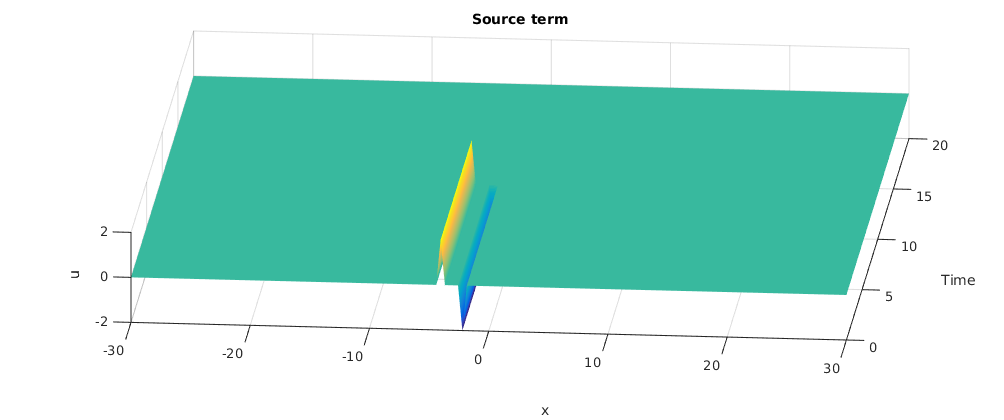
\includegraphics[width = 0.45\textwidth]{images/initcontrol.png}
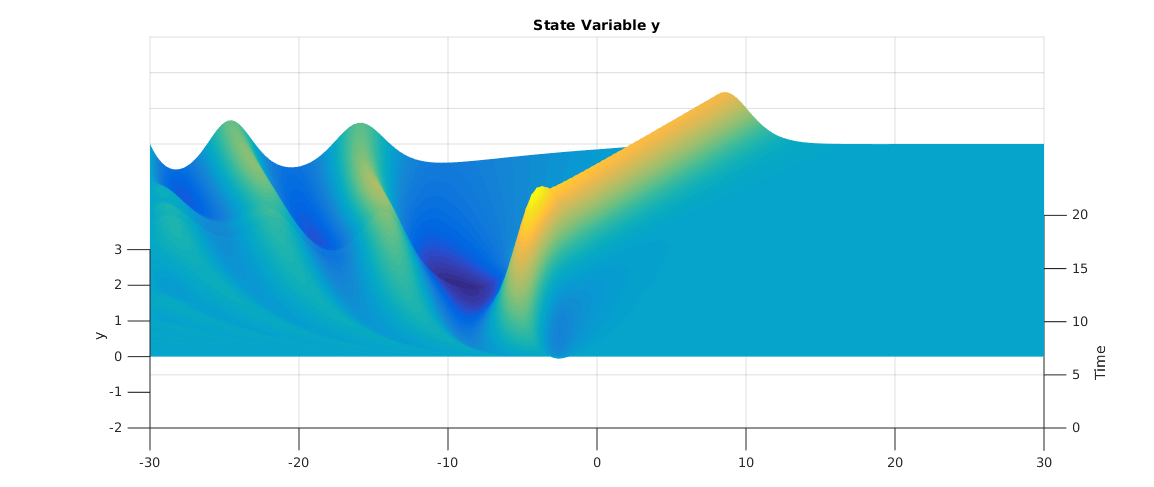
\includegraphics[width = 0.45\textwidth]{images/waveobservation.png}
\caption{Left: forcing term as in \eqref{forcingq}. Right : wave generated by the forcing term $u$, for $f = -0.5$ (i.e. subcritical flow).}
\label{waveobservation}
\end{figure}
One can see a series of downstream waves generated by the bottom topography induced by $u$ (recall that $u$ is proportional to the derivative of the topography), while a solitary wave is going upstream, at constant speed and constant height, which is typical for the Korteweg-de Vries equation. We want to track the shape of the water surface on $\Omega_{obs}$ while acting only on the control domain $\Omega_c$.

\begin{figure}[!h]
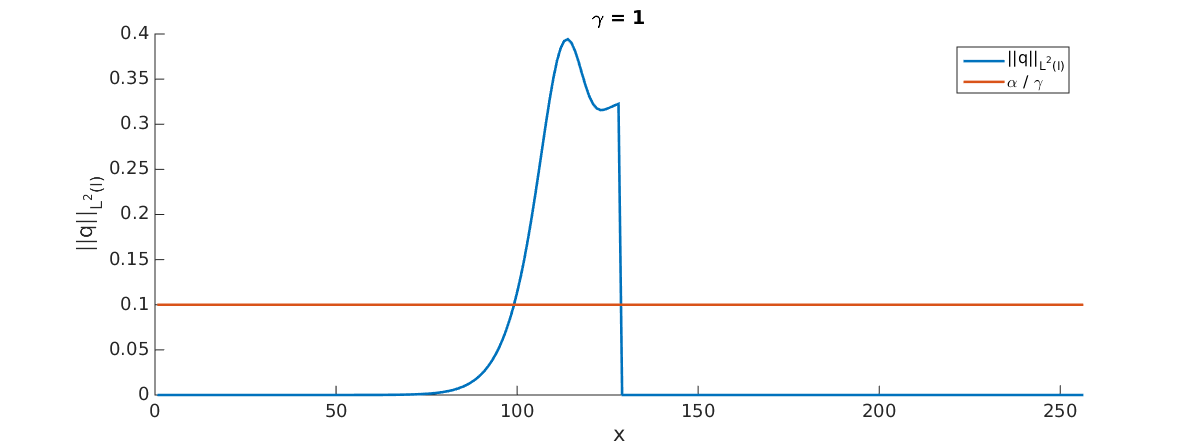
\includegraphics[width = 0.45\textwidth]{images/normq1.png}
%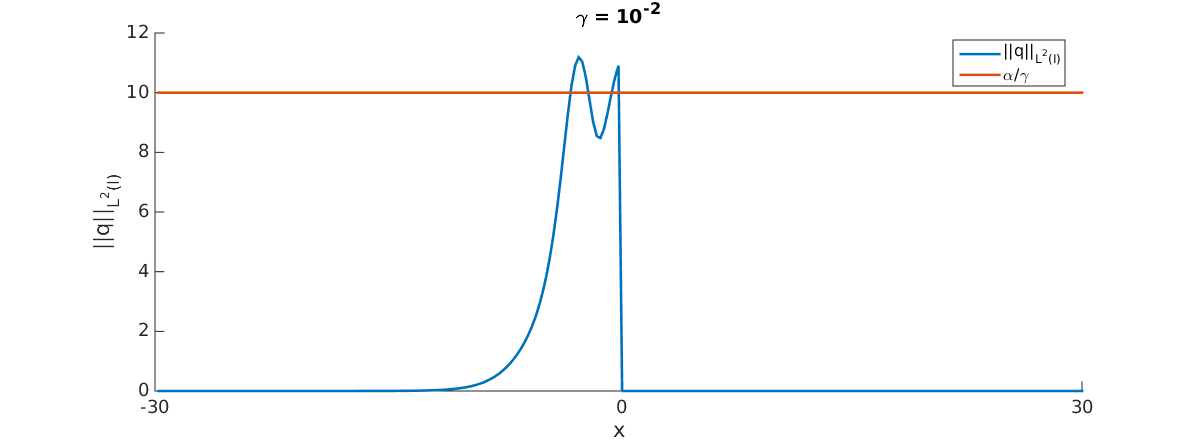
\includegraphics[width = 0.45\textwidth]{images/normq100.png}
%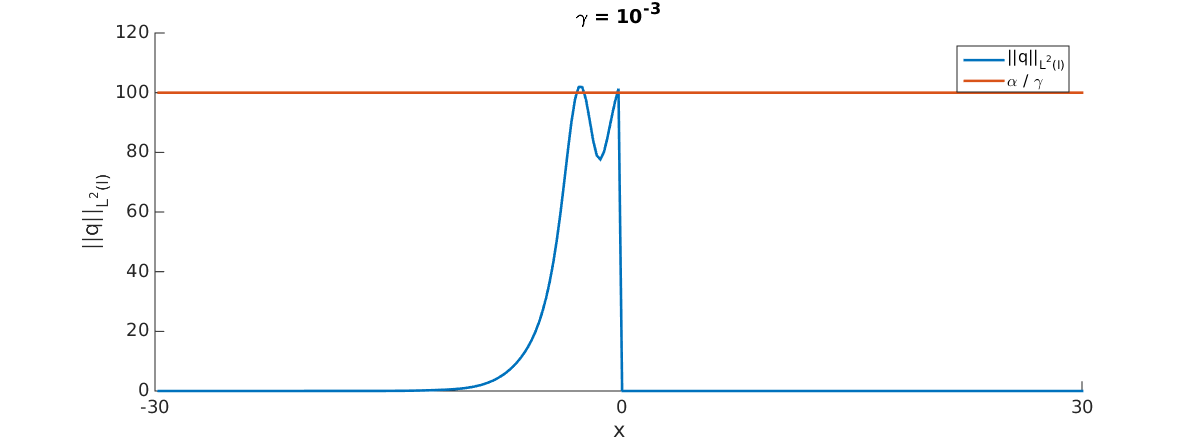
\includegraphics[width = 0.45\textwidth]{images/normq1000.png}
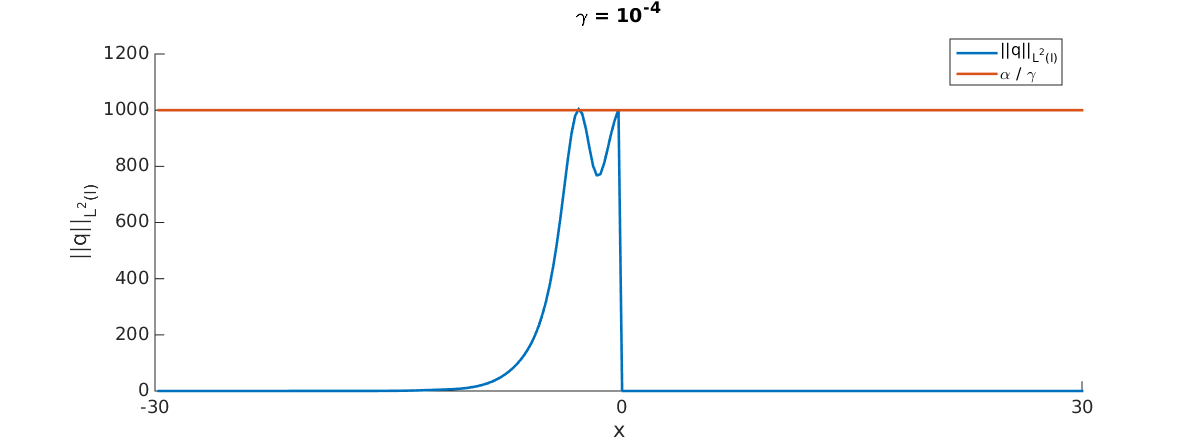
\includegraphics[width = 0.45\textwidth]{images/normq10000.png}
\caption{Evolution of the support of the control, determined by $\norm{q}_{L^2(0,T)}\geq \frac{\alpha}{\gamma}$.}
\label{waveobservation}
\end{figure}

\begin{figure}[!h]
 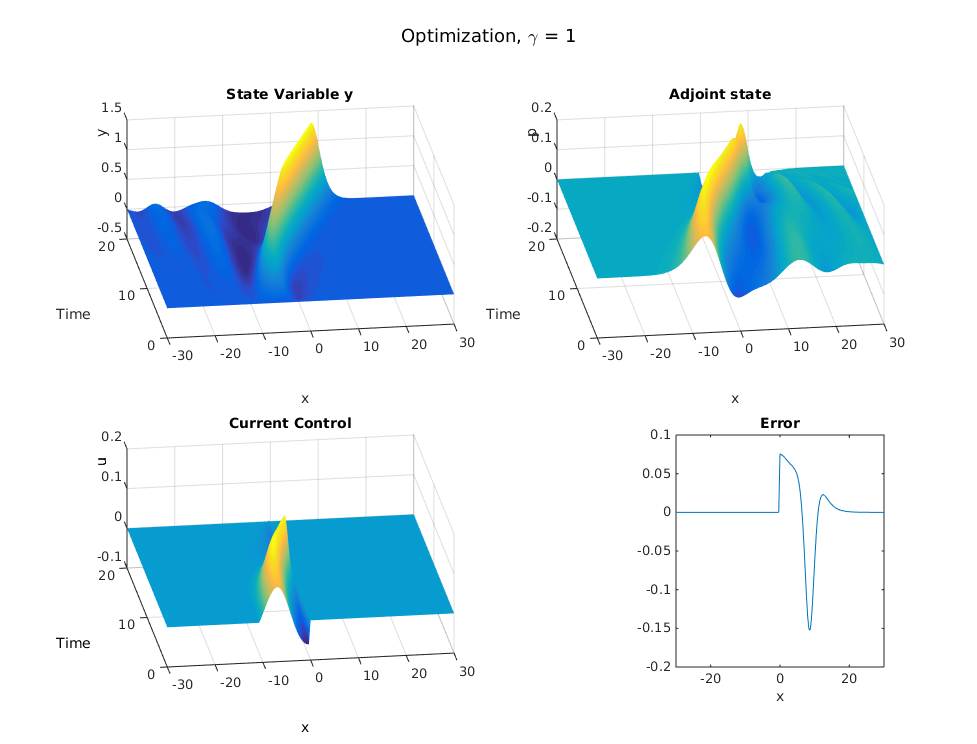
\includegraphics[width = 0.8\textwidth]{images/gamma1results.png}
 \caption{State y, adjoint state p and control at the end of the optimization procedure for $\gamma = 1$}
\end{figure}

% \begin{figure}[!h]
%  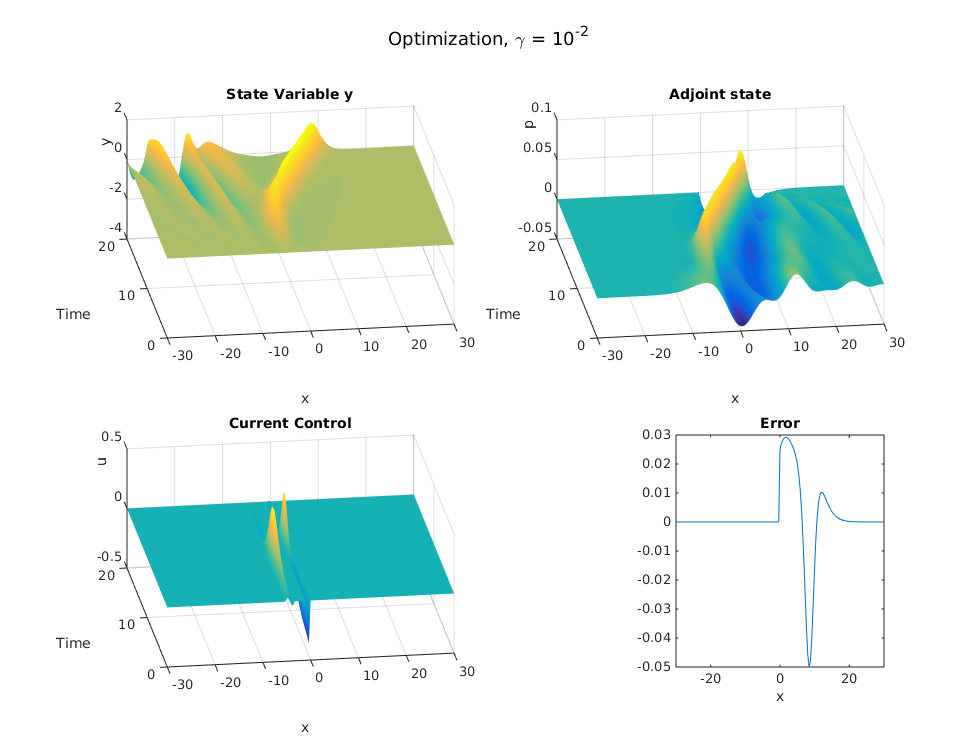
\includegraphics[width = 0.8\textwidth]{images/gamma100results.png}
%  \caption{State y, adjoint state p and control at the end of the optimization procedure for $\gamma = 1$}
% \end{figure}
% 
% \begin{figure}[!h]
%  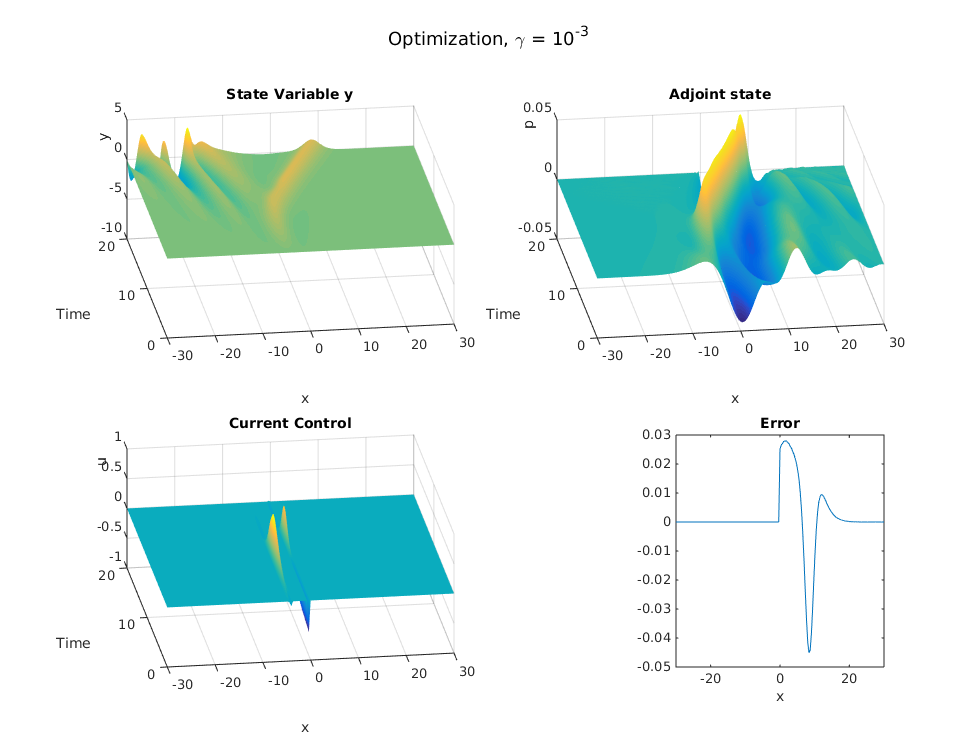
\includegraphics[width = 0.8\textwidth]{images/gamma1000results.png}
%  \caption{State y, adjoint state p and control at the end of the optimization procedure for $\gamma = 1$}
% \end{figure}

\begin{figure}[!h]
 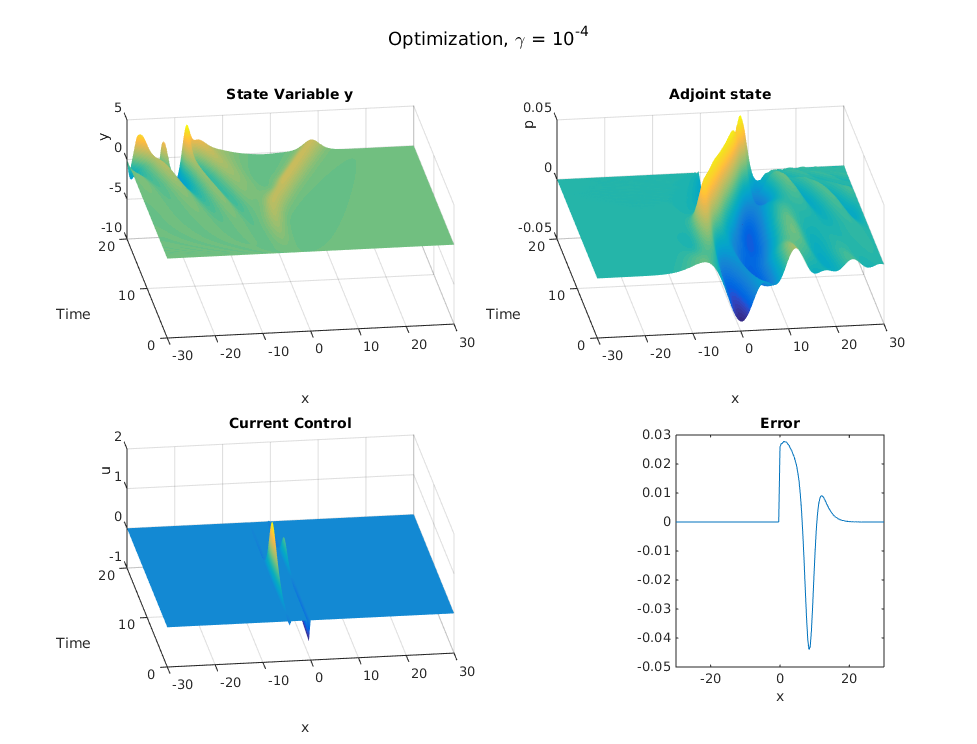
\includegraphics[width = 0.8\textwidth]{images/gamma10000results.png}
 \caption{State y, adjoint state p and control at the end of the optimization procedure for $\gamma = 10^{-4}$}
\end{figure}







%%% Local Variables: 
%%% mode: latex
%%% TeX-master: "kdv.tex"
%%% End:

\section*{Acknowledgement}
The authors warmly thank Tang Quoc Bao, Felix Henneke, Karl Kunisch, Konstantin Pieper and Boris Vexler for fruitful discussions during this work. %Also, the authors gratefully acknowledge support from the International Research Training Group IGDK 1754, funded by the German Science Foundation (DFG) and Austrian Science Foundation (FWF).
\appendix
\section{Well-posedness of the state equation}
\label{sec:appwp}

% \subsection{Semigroup of contractions}
% \label{sec:semigr-contr}
% \begin{proof}[Proof of Proposition~\ref{propsemigroup}]
%   The idea of the proof is not new and was first introduced in \cite{rosier1997exact}. We choose to provide it here as we are concerned with a slightly different operator (we add diffusion to the problem).
%   The idea is to prove that $A$ is maximally dissipative in order to
%   use a corollary of the Lumer-Philips theorem and conclude. We
%   already have that $A:\mathcal{D}(A) \mapsto L^{2}(0,L)$ has a dense
%   domain and it is easy to see that it is a closed operator. Let us
%   prove that it is dissipative. For any $w \in \mathcal{D}(A)$, \beal
%   <w,Aw>_{L^{2}(0,L)} &= \int_{0}^{L}{w(-w'''-w'+\gamma w'')dx}\\
%   & = -[ww'']_{0}^{L} + \int_{0}^{L}{w'w''dx} - [w^{2}]_{0}^{L} + \gamma [ww']_{0}^{L} - \gamma \int_{0}^{L}{w'^{2}dx}\\
%   & = -\frac{1}{2}w'(0)^{2} - \gamma \int_{0}^{L}{w'^{2}dx} \leq 0.
%   \eeal Hence A is dissipative. Denoting $A^{\ast}$ the adjoint
%   operator of $A$ satisfying \be A^{\ast}w = w''' + w' + \gamma w'',
%   \ee we also have \beal
%   <A^{\ast}w,w>_{L^{2}(0,L)} &= \int_{0}^{L}{w(w'''+w'+\gamma w'')dx}\\
%   & = -\frac{1}{2}w'(L)^{2} - \gamma \int_{0}^{L}{w'^{2}dx} \leq 0.
%   \eeal Therefore $A^{\ast}$ is also dissipative and A is maximally
%   dissipative. A corollary of the Lumer-Philips theorem theorem (see
%   \cite{pazy1983semigroups}, Chapter 1, Cor 4.4) permits to conclude
%   that A generates a strongly continuous semigroup of contractions.
% \end{proof}

\subsection{Linear estimates}
\label{sec:linear-estimates}
\begin{proof}[Proof linear estimate \eqref{linestimate_regular}]
  The proof is here largely inspired from \cite{rosier1997exact,glass2008some}. Let $y\in \mathcal C(\bar I,\mathcal D(A))~\cap~\mathcal C^1(\bar I,L^2(\Omega))$ be the classical solution of \eqref{kdvlinnonhom} for data $f\in \Hm1$ and $y_0\in \mathcal D(A)$. We multiply \eqref{kdvlinnonhom1} which holds in $L^2(\Omega)$ for a.e. $t\in I$ with $y$ and get
   \be
  \frac{1}{2}\frac{d}{dt}\int_{0}^{L}{y^{2}dx} + \abs{\partial_{x}y(t,0)}^{2} + \gamma \int_{0}^{L}{(\partial_{x} y)^{2}dx}=  \langle f,y\rangle_{H^{-1}(\Omega),H^{1}_{0}(\Omega)}.
  \ee
  Applying Cauchy-Schwarz followed by Young's inequality to the right-hand side
  leads to \be \frac{1}{2}\frac{d}{dt}\int_{0}^{L}{y^{2}dx} + \abs{\partial_{x} y(t,0)}^{2} + \gamma \int_{0}^{L}{(\partial_{x}y)^{2}dx}\leq \frac{1}{2}\norm{f}_{H^{-1}(\Omega)}^{2} + \frac{1}{2}\norm{y}_{H^{1}_{0}(\Omega)}^{2}
  \label{linnhupperbound1}.
  \ee
  We proceed in the same manner testing with $xy$
  \be
  \frac{1}{2}\frac{d}{dt}\int_{0}^{L}{xy^{2}dx}-\frac{1}{2}\int_{0}^{L}{y^{2}dx} +  \frac{3}{2}\int_{0}^{L}{(\partial_{x} y)^{2}dx} +\gamma
  \int_{0}^{L}{x(\partial_{x} y)^{2}dx}= \langle f,xy \rangle_{H^{1}_{0}(\Omega)}.
  \label{linnhupperbound2}
  \ee
  The right-hand side is treated again thanks to Cauchy-Schwarz
  and Young's inequalities
  \beal
  \langle f,xy\rangle_{H^{-1}(\Omega),H^{1}_{0}(\Omega)} &\leq \norm{q}_{H^{-1}(\Omega)}\norm{xy}_{H^{1}_{0}(\Omega)}\\
  & \leq \norm{f}_{H^{-1}(\Omega)}\norm{y + x\partial_{x}y}_{L^{2}(\Omega)}\\
  % & \leq \norm{q}_{H^{-1}(\Omega)} \left( \norm{y}_{L^{2}(\Omega)} + \norm{x\partial_{x}y}_{L^{2}(\Omega)} \right)\\
  & \leq \norm{f}_{H^{-1}(\Omega)} \left( \norm{y}_{L^{2}(\Omega)} + L\norm{\partial_{x}y}_{L^{2}(\Omega)} \right)\\
  &\leq \frac{1}{2}\norm{f}_{H^{-1}(\Omega)}^{2} + \frac{1}{2}\norm{y}_{L^{2}(\Omega)}^{2} + \frac{L^{2}}{2}\norm{f}_{H^{-1}(\Omega)}^{2} + \frac{L}{2L}\norm{\partial_{x}y}_{L^{2}(\Omega)}^{2}\\
  &\leq \frac{1+L^{2}}{2}\norm{f}_{H^{-1}(\Omega)}^{2} +  \frac{1}{2}\norm{y}_{L^{2}(\Omega)}^{2} +  \frac{1}{2}\norm{\partial_{x}y}_{L^{2}(\Omega)}^{2}
  \label{upperboundq}
  \eeal
  Adding \eqref{linnhupperbound1}, \eqref{linnhupperbound2}(with the upper bound \eqref{upperboundq}) and omitting some non-negative terms on the left-hand side yields \be
  \frac{1}{2}\frac{d}{dt}\int_{0}^{L}{(1+x)y^{2}dx} +(\frac{1}{2}+\gamma)\int_{0}^{L}{(\partial_{x}y)^{2}} \leq \left(   1 +\frac{L^{2}}{2}\right)\norm{f}_{H^{-1}(\Omega)}^{2} + \int_{0}^{L}{y^{2}dx}.
  \ee
   To facilitate the next computations, we add a non-negative term on the right and multiply by two
   \be
 \frac{d}{dt}\int_{0}^{L}{(1+x)y^{2}dx} + (1+2\gamma)\int_{0}^{L}{(\partial_{x}y)^{2}} \leq \left(    2 +L^{2}\right)\norm{f}_{H^{-1}(\Omega)}^{2} +  2\int_{0}^{L}{(1+x)y^{2}dx}.
  \ee
  Then we can follow a Gronwall strategy, multiplying by $e^{-t}$
  \beal
  \frac{d}{dt}\left(e^{-2t}\int_{0}^{L}{(1+x)y^{2}dx}\right) + e^{-2t}\left(1+2\gamma\right)\int_{0}^{L}{(\partial_{x}y)^{2}} \leq
  e^{-2t}\left( 2+L^{2}\right)\norm{f}_{H^{-1}(\Omega)}^{2}
  \eeal
  After integration between $0$ and $t$  and multiplication by $e^{2t}$we have
  \beal
  \int_{0}^{L}{y^{2}(t)dx} + \left( 1+2\gamma \right)\int_{0}^{t}{\int_{0}^{L}{(\partial_{x} y)^{2}dxdt}} \leq e^{2t}\left(2+L^{2}\right)&\int_{0}^{t}{\norm{f}_{H^{-1}(\Omega)}^{2}}\\
  & + e^{2t}\int_{0}^{L}{(1+L)y_{0}^{2}dx},
  \eeal
  that we transform into
  \beal
  \int_{0}^{L}{y^{2}(t)dx} + \left( 1+2\gamma \right)\int_{0}^{t}{\int_{0}^{L}{(\partial_{x} y)^{2}dxdt}} \leq e^{2T}\left(2+L^{2}\right)&\norm{f}_{L^{2}(I,H^{-1}(\Omega))}^{2} \\
  &+ e^{2T}(1+L)\norm{y_{0}}_{L^{2}(\Omega)}.
  \eeal
  This yields
  \[\|y\|_{\mathcal C(\bar I,L^2(\Omega))}+\|y\|_{L^2(I,H^1_0(\Omega))}\leq c(\|f\|_{\Hm1}+\|y_0\|_{L^2(\Omega)}).\]



  %Because
%  it is a one-dimensional problem, there holds
%$$\M \hookrightarrow L^{2}(I, \mathcal{M}(\Omega)) \hookrightarrow L^{2}(I, H^{-1}(\Omega)).$$
%Therefore we obtain estimate \eqref{linestimate} for any $y_{0} \in
%\mathcal{D}(A)$ and $q \in C_{0}([0,T], \mathcal{D}(A))$. Let us
%conclude by a density argument. We consider two sequences
%$$ y_{0}^{n} \in \mathcal{D}(A) \xrightarrow[n\rightarrow+\infty]{}y_{0} \in L^{2}(\Omega),\quad
%q^{n} \in  C_{0}([0,T], \mathcal{D}(A)) \xrightarrow[n\rightarrow+\infty]{} q \in L^{2}(I,H^{-1}(\Omega)).$$
%We associate to any pair $\left(y_{0}^{n}, q^{n}\right)$ the sequence
%of solutions $(y^{n})$. Due to the linearity of the considered
%equation, the estimate \eqref{linestimate} implies that $(y^{n})$ is a
%Cauchy sequence in $\mathcal{B}$ that converges towards some $y \in
%\mathcal{B}$. Besides, uniqueness follows from semigroup theory and
%uniqueness of the limit. This concludes the proof.
\end{proof}

% \subsection{Weak formulation}
% \label{sec:weak-formulation}
% \begin{proof}[Proof for Remark~\ref{rmkweakform}]
%   In the proof of Proposition~\ref{propnonhomo}, the solution $y$ to \eqref{kdvlinnonhom} is defined as the limit in $\mathcal{B}$ of the smooth solution $y^n$ of \eqref{kdvlinnonhom} obtained for smooth initial conditions and right-hand side
% \beal
% & y_0^n \in \mathcal{D}(A)\underset{n\to +\infty}{\longrightarrow} y_0 \in L^2(\Omega),\quad
% & q_n \in C(0,T,\mathcal{D}(A))\underset{n\to +\infty}{\longrightarrow}q \in \M.
% \eeal
% This solution $y^n$, because of its regularity, clearly satisfies \eqref{kdvlinnonhom} in a classical sense, a fortiori in the sense of \eqref{weakform}, obtained after successive integrations by part
% \be
% -(y^n,\partial_t \varphi)_I + (\partial_x y^n, \varphi)_I + (\partial_x y^n, \partial_{xx}\varphi)_I + \gamma (\partial_x y^n, \partial_x \varphi)_I = <q^n,\varphi>, \quad \forall \varphi \in \mathcal{V}.
% \ee
% Then, for each term, using on the one hand the embeddings $\mathcal{V}\hookrightarrow L^2(I,H^2\cap H^1_0)\hookrightarrow L^2(I, L^2(\Omega))$, and on the other hand the regularity of $y$, one can write
% \beal
% \abs{(y^n-y,\partial_t \varphi)_I}\leq \norm{y^n - y}_{L^2(I\times\Omega)} \norm{\partial_t \varphi}_{L^2(I\times\Omega)} &\leq \norm{y^n - y}_{L^2(I,H^1_0(\Omega))} \norm{ \varphi}_{H^1(0,T,L^2(\Omega))}\\
% &\leq \norm{y^n - y}_{\mathcal{B}} \norm{\varphi}_{\mathcal{V}}
% \eeal
%
% \beal
% \abs{(\partial_x (y^n-y),\varphi)_I}\leq \norm{\partial_x (y^n - y)}_{L^2(I\times\Omega)} \norm{\varphi}_{L^2(I\times\Omega)} &\leq \norm{y^n - y}_{L^2(I,H^1_0(\Omega))} \norm{\varphi}_{\mathcal{V}} \\
% &\leq \norm{y^n - y}_{\mathcal{B}} \norm{\varphi}_{\mathcal{V}}
% \eeal
%
% \beal
% \abs{(\partial_x( y^n-y),\partial_{xx} \varphi)_I}\leq \norm{\partial_x (y^n - y)}_{L^2(I\times\Omega)} \norm{\partial_{xx} \varphi}_{L^2(I\times\Omega)} &\leq \norm{y^n - y}_{L^2(I, H^1_0(\Omega))}\norm{\varphi}_{L^2(I, H^2 \cap H^1_0(\Omega))}\\
% & \leq \norm{y^n - y}_{\mathcal{B}} \norm{\varphi}_{\mathcal{V}}
% \eeal
%
% \beal
% \abs{(\partial_x (y^n-y),\partial_x \varphi)_I}\leq \norm{\partial_x( y^n-y)}_{L^2(I\times\Omega)} \norm{\partial_x \varphi}_{L^2(I\times\Omega)} &\leq  \norm{y^n - y}_{L^2(I, H^1_0(\Omega))} \norm{\varphi}_{L^2(I, H^1_0(\Omega))}\\
% &\leq \norm{y^n - y}_{\mathcal{B}} \norm{\varphi}_{\mathcal{V}}
% \eeal
% Recall that $\norm{y^n - y}_{\mathcal{B}} \norm{\varphi}_{\mathcal{V}} \underset{n\to +\infty}{\longrightarrow} 0$. Moreover, since $q^n$ tends to $q$ in $L^2(I,H^{-1}(\Omega))$, one directly has
% \be
% <q^n,\varphi> \underset{n\to +\infty}{\longrightarrow} <q,\varphi>.
% \ee
% As a consequence, $y$ satisfies
% \be
% -(y,\partial_t \varphi)_I + (\partial_x y, \varphi)_I + (\partial_x y, \partial_{xx}\varphi)_I + \gamma (\partial_x y, \partial_x \varphi)_I = <q,\varphi>, \quad \forall \varphi \in \mathcal{V}.
% \ee
% \end{proof}



\subsection{Nonlinear state equation}
\label{sec:nonl-state-equat}
\begin{proof}[Proof of Lemma~\ref{lemyyx2}] The technique is inspired from (\cite{faminskii2010initial}, Proof of Theorem 2.8). Let us consider $y \in \B$ and $z \in \B$. It holds $\mathcal B\hookrightarrow L^4(I\times \Omega)$ and therefore we can estimate using $\|y\|_{L^\infty(\Omega)}^2\leq c\|y\|_{L^2(\Omega)}\|y\|_{H^1_0(\Omega)}$
\beal
\norm{y\partial_x y - z\partial_x z}_{\Hm1}  & = \frac 1 2\left(\int_0^T{\left(\ \sup_{\norm{\varphi}_{H^1_0(\Omega) = 1}}(y^2 -  z^2,\partial_x\varphi)_{L^2(\Omega)}\right)^2}\mathrm dt\right)^{1/2} \\
& \leq \frac{1}{2}\norm{z-y}_{L^4(I\times \Omega)}\norm{z+y}_{L^4(I\times \Omega)} \\
& \leq\frac{1}{2} \norm{z-y}_{C(0,T,L^2(\Omega))}^{1/2}\left( \int_0^T{\norm{z-y}_{L^{\infty}(\Omega)}^2}\right)^{1/4}\\
&\quad \quad\cdot\norm{z+y}_{C(0,T,L^2(\Omega))}^{1/2}\left( \int_0^T{\norm{z+y}_{L^{\infty}(\Omega)}^2}\right)^{1/4}\\
& \leq c\, \norm{z-y}_{C(0,T,L^2(\Omega))}^{1/2}\norm{z+y}_{C(0,T,L^2(\Omega))}^{1/2}\\
& \quad \quad\cdot \left(\int_0^T{ \norm{z-y}_{L^2(\Omega)}\norm{z-y}_{H^1_0(\Omega)}}\right)^{1/4}\left(\int_0^T{ \norm{z+y}_{L^2(\Omega)}\norm{z+y}_{H^1_0(\Omega)}}\right)^{1/4}\\
& \leq c \,T^{1/4}\norm{z-y}_{C(0,T,L^2(\Omega))}^{3/4}\norm{z-y}_{L^2(0,T,H^1_0(\Omega))}^{1/4}\\
& \quad \quad \cdot\norm{z+y}_{C(0,T,L^2(\Omega))}^{3/4}\norm{z+y}_{L^2(0,T,H^1_0(\Omega))}^{1/4} \\
&\leq c \,T^{1/4}\norm{y-z}_{\B}\norm{y+z}_{\B}
\eeal
\end{proof}

%\begin{proof}[Proof of Proposition~\ref{localposedness}, uniqueness]
%We now prove the uniqueness of the (weak) solution of the nonlinear KdV equation \eqref{kdvcontrol1} - \eqref{kdvcontrol3}. Let us first consider two solutions of the same Cauchy problem $y$ and $z$ defined on $[0,T^{\ast}]\times\Omega$. Then $u = y-z$ is a solution of
%\bealn
%&\partial_t u +\partial_x u + \partial_{xxx} u -\gamma \partial_{xx} u= - y\partial_x u - u\partial_x z \mbox{ in }   I\times\Omega,\\
%&u(.,0) = u(.,L) = \partial_x u (.,L) = 0 \mbox{ on } I\times\Gamma,\\
%&u(0,.) = 0 \mbox{ in } \Omega,
%\label{kdvnonlin1}
%\eealn
%Multiplying by $2xu$ and integrating in $x$ (as proposed in \cite{rosier1997exact,coron2003exact}) leads to
%\be
%\int_{0}^{L}{2xu\left( \partial_t u +\partial_x u + \partial_{xxx} u -\gamma \partial_{xx} u+ y\partial_x u + u\partial_x z\right)dx} = 0,
%\ee
%which also writes
%\be
%\frac{d}{dt}\int_{0}^{L}{xu^2dx} + 3\int_0^L{(\partial_x u)^2dx} +  2\gamma\int_0^L{x(\partial_x u)^2dx} = \int_0^L{u^2dx} - 2\int_0^L{x y u \partial_x udx} + 2\int_0^L{zu^2 dx}+4\int_0^L{x z u \partial_x u dx}
%\ee
%Then, we follow \cite{coron2003exact} to upperbound every term on the right hand side. Thanks to the continuous embedding of $H^1_0(\Omega)$ into $C^0(\Omega)$, there exists a positive constant $C$ such that
%\be
%2\megaabs{\int_0^L{xy u \partial_x u dx}} \leq C_1 \norm{\partial_x y}_{L^2(\Omega)}\int_0^L{\abs{x u \partial_x u}dx}
%\label{eq1}
%\ee
%Using Cauchy-Schwarz and Young's inequalities leads to
%\be
%2\megaabs{\int_0^L{xy u \partial_x u dx}} \leq \frac{1}{2}\int_0^L{\left(\partial_x u\right)^2dx} + \frac{C_1^2}{2}\norm{\partial_x y}_{L^2(\Omega)}^2 L\int_0^L{x u^2 dx}.
%\label{eq2}
%\ee
%And the same process is applied to
%\be
%4\megaabs{\int_0^L{x z u \partial_x u dx}} \leq \frac{1}{2}\int_0^L{\left(\partial_x u\right)^2dx} + 2 C_1^2\norm{\partial_x z}_{L^2(\Omega)}^2 L\int_0^L{x u^2 dx}.
%\label{eq3}
%\ee
%Recalling from \cite{coron2003exact} the lemma
%\begin{lem}
%For every $\phi \in H^1_0(0,L)$ with $\phi(0) = 0$ and every $a \in [0,L]$,
%\be
%\int_0^L{\phi^2dx} \leq \frac{a^2}{2}\int_0^L{\left(\partial_x \phi \right)^2 dx} + \frac{1}{a}\int_0^L{x\phi^2 dx},
%\ee
%\label{lem1}
%\end{lem}
%\noindent one can prove that there exists $C_{2}$ such that
%\be
%\int_0^L{u^{2}dx} \leq \frac{1}{2}\int_{0}^{L}{\left( \partial_{x}u\right)^{2}dx} + C_{2}\int_{0}^{L}{xu^{2}dx}.
%\label{eq4}
%\ee
%Finally, using the same justification as \eqref{eq1}, there exists $C_{3}$ such that
%\be
%2\megaabs{\int_0^L{zu^{2} dx}} \leq C_{3}\norm{z_{x}}_{L^{2}(0,L)}\int_{0}^{L}{u^{2}dx},
%\ee
%Combined with \eqref{eq4}, this latter inequality rewrites, for a constant $C_{4}$
%\be
%2\int_0^L{zu^{2} dx} \leq \frac{1}{2}\int_{0}^{L}{\left( \partial_{x} u\right)^{2}dx} + C_{4} \left( 1 + \norm{z_{x}}_{L^{2}(0,L)}^{3/2}\right) \int_{0}^{L}{xu^{2}dx}
%\label{eq5}
%\ee
%Now, by \eqref{eq2}, \eqref{eq3}, \eqref{eq4}, \eqref{eq5}, we have
%\beal
%\frac{d}{dt}\int_{0}^{L}{xu^2dx} + \int_0^L{(\partial_x u)^2dx} \leq C_5 \left( 1 + \norm{\partial_x y}_{L^2(\Omega)}^2 + \norm{\partial_x z}_{L^2(\Omega)}^2 \right)\int_0^L{ xu^2 dx}
%\label{eq6}
%\eeal
%for a given constant $C_5$.
%In particular, applying Gronwall lemma to
%\be
%\frac{d}{dt}\int_{0}^{L}{xu^2dx} \leq C_5 \left( 1 + \norm{\partial_x y}_{L^2(\Omega)}^2 + \norm{\partial_x z}_{L^2(\Omega)}^2 \right)\int_0^L{ xu^2 dx}
%\ee
%leads to
%\be
%\int_{0}^{L}{xu^2dx} \leq \left[\int_{0}^{L}{xu_0^2dx}\right]\, e^{\displaystyle \int_0^s{C_5 \left( 1 + \norm{\partial_x y}_{L^2(\Omega)}^2 + \norm{\partial_x z}_{L^2(\Omega)}^2 \right)ds}} = 0,
%\label{eqend}
%\ee
%since in our case $u_0 = 0$, \eqref{eqend} leads to $u = 0$ in $C^0(I,L^2(\Omega))$. Moreover, using again \eqref{eq6}
%we have
%\be
%\int_0^{T^{\ast}}{\int_0^L{(\partial_x u)^2dx}} \leq \int_0^{T^{\ast}}{C_5 \left( 1 + \norm{\partial_x y}_{L^2(\Omega)}^2 + \norm{\partial_x z}_{L^2(\Omega)}^2 \right)\int_0^L{ xu^2 dx}} = 0,
%\ee
%which leads also to $u = 0$ in $L^2(I, H^1_0(\Omega))$. Unicity of the solution to the nonlinear KdV system is thus proved.
%\end{proof}

\subsection{The tangent equation}\label{appendixtangent}
Next we analyze be well posedness of the tangent equation
\begin{subequations}
 \begin{numcases}{}
\partial_t \delta y +\partial_x \delta y + \partial_{xxx} \delta y - \gamma \delta \partial_{xx} y  + \partial_x(y \delta y)=  \delta q \mbox{ in } I\times\Omega,\label{linkdv1}\\
\delta y(.,0) = \delta y(.,L) = \partial_x \delta y (.,L) = 0 \mbox{ in } I,\label{linkdv2}\\
\delta y(0,x) = \delta y_0 \mbox{ in } \Omega.\label{linkdv3}
 \end{numcases}
\end{subequations}
\begin{Def}
Let $(\delta q,\delta y_0)\in\M\times \mathcal B$ and $y\in \mathcal B$. A function $\delta y\in \mathcal B$ is called a solution of \eqref{linkdv1}-\eqref{linkdv3} if it satisfies the fixed point equation
\[
\delta y=\mathcal L(\delta q-\partial_x(y\delta y),\delta y_0)
\]
where $\mathcal L$ is the solution operator from Remark \ref{rmklinearoperator}.
\end{Def}
\begin{prop}\label{prop:tangent}
 Let $(\delta q,\delta y_0) \in \Hm1\times L^2(\Omega)$ and $y\in \mathcal B$. Then, there exists a unique solution $\delta y \in \mathcal{B}$ of \eqref{linkdv1}-\eqref{linkdv3}. Furthermore, there exists a constant $\widetilde C(T,L,\norm{y}_{\mathcal{B}})$ such that the following estimate holds
 \be\label{estimatetangent}
 \norm{\delta y}_{\mathcal B}+\|\partial_t \delta y\|_{L^2(I,\mathcal V^*)} \leq \widetilde C \left( \norm{\delta y_0}_{L^2(\Omega)} + \norm{\delta q}_{\Hm1}\right).
 \ee
\end{prop}
\begin{proof}[Proof of Proposition~\ref{prop:tangent}]
We define the linear mapping
\[
\Psi_{\delta q, \delta y_0,y}\colon \mathcal B_{\theta}\rightarrow B_{\theta},~~\Psi_{\delta q, \delta y_0,y}(\delta y) = \mathcal{L}(\delta q - \partial_x(y\delta y),\delta y_0)
\]
with $\mathcal B_{\theta}$ defined as in \eqref{btheta} and \eqref{normbtheta} and $\mathcal{L}$ being the linear \KdV operator described in Remark~\ref{rmklinearoperator}. Our goal is to show that under some constraints on $\theta$, $\Psi_{\delta q, \delta y_0,y}$ is a contraction mapping, such that the Banach fixed point theorem can be applied. First we estimate $\partial_x(y \delta y)$ in the $L^2([0,\theta],H^{-1}(\Omega))$-norm
\beal\label{estimate_variable_coefficient}
\|\partial_x(y\delta y)\|_{L^2([0,\theta],H^{-1}(\Omega))} &\leq \left(\int_{0}^{\theta}\left(\underset{\|v\|_{H^1_0(\Omega)}\leq 1}{\operatorname{sup}}\langle\partial_x(y\delta y)(t),v\rangle_{H^{-1}(\Omega),H^1_0(\Omega)}\right)^2~\mathrm dt\right)^{\frac{1}{2}}\\
&\leq\left(\int_{0}^{\theta}\|\delta y(t)\|_{L^2(\Omega)}^2\|y(t)\|_{L^\infty(\Omega)}^2~\mathrm dt\right)^{\frac{1}{2}}\\
&\leq c\,\|\delta y\|_{\mathcal C([0,\theta],L^2(\Omega))}\left(\int_{0}^{\theta}\|y(t)\|_{H^1_0(\Omega)}\|y(t)\|_{L^2(\Omega)}~\mathrm dt\right)^{\frac{1}{2}}\\
&\leq c\,\theta\,\|\delta y\|_{\mathcal C([0,\theta],L^2(\Omega))}\left(\int_{0}^{\theta}\|y(t)\|_{H^1_0(\Omega)}^2\|y(t)\|_{L^2(\Omega)}^2~\mathrm dt\right)^{\frac{1}{2}}\\
&\leq c\,\theta\,\|\delta y\|_{\mathcal C([0,\theta],L^2(\Omega))}\|y\|_{\mathcal C([0,\theta],L^2(\Omega))}\|y\|_{L^2([0,\theta],H^1_0(\Omega))}\\
&\leq c\,\theta\,\|y\|_{\mathcal B_{\theta}}^2\|\delta y\|_{\mathcal B_{\theta}}
\eeal
Therefore we can estimate
\beal
\|\Psi(\delta y)_{\delta q, \delta y_0,y}\|_{\mathcal B_{\theta}} & \leq \widetilde{C}\left(\|\delta y_0\|_{L^2(\Omega)}+\|\delta q\|_{L^2(I,H^{-1}(\Omega))}+\|\partial_x(y\delta y)\|_{L^2([0,\theta],H^{-1}(\Omega))}\right)\\
&\leq \widetilde{C}\left(\|\delta y_0\|_{L^2(\Omega)}+\|\delta q\|_{L^2(I,H^{-1}(\Omega))}\right) + C_2\theta\|y\|_{\mathcal B_{\theta}}^2\|\delta y\|_{\mathcal B_{\theta}}
\eeal
and
\be
\|\Psi_{\delta q, \delta y_0,y}(\delta y_1)-\Psi_{\delta q, \delta y_0,y}(\delta y_2)\|_{\mathcal B_{\theta}}\leq C_2\theta\|y\|_{\mathcal B_{\theta}}^2\|\delta y_1-\delta y_2\|_{\mathcal B_{\theta}}.
\ee
Now we set $r=2 \widetilde{C}\left(\|\delta y_0\|_{L^2(\Omega)}+\|\delta q\|_{L^2(I,H^{-1}(\Omega))}\right)$ and introduce the ball
\[
B=\{\delta y \in \mathcal B_{\theta}\colon \|\delta y\|_{\mathcal B_{\theta}}\leq r\}.
\]
Next we choose $\theta$ small enough such that
\[
C_2\theta\|y\|_{\mathcal B}^2\leq\frac{1}{3}
\]
holds. Then the following inequalities hold
\[
\|\Psi_{\delta q, \delta y_0,y}(\delta y)\|_{\mathcal B_{\theta}}\leq \frac{2}{3}r,~~\|\Psi_{\delta q, \delta y_0,y}(\delta y_1) - \Psi_{\delta q, \delta y_0,y}(\delta y_2)\|_{\mathcal B_{\theta}}\leq\frac{2}{3}\|\delta y_1-\delta y_2\|_{\mathcal B_{\theta}}.
\]
which implies that $\Psi_{\delta q, \delta y_0,y}$ is a contraction mapping on $B$. So we can apply the Banach fixed point theorem which guarantees the existence of a unique fixed point $\delta y$ of $\Psi_{\delta q, \delta y_0,y}$ which is a solution of \eqref{linkdv1}-\eqref{linkdv3} in $(0,\theta)$ with initial value $\delta y_0$. Since $\theta$ is independent of $\delta y_0$ we can apply this strategy successively starting at $t=0$ with $\delta y_0$ and using $\delta y(k\theta)$ as initial points for $k=1,2,3,\ldots,N$ until $T$ is reached. The concatenation of all $\delta y(k\theta)$ for $k=1,2,3,\ldots,N$ is a solution of \eqref{linkdv1} - \eqref{linkdv3}. Existence of a unique solution is thus proven. Concerning the estimates \eqref{estimatetangent}, the proof is very similar to the non-variable coefficients case (see Appendix~\ref{sec:linear-estimates}). We just mention the main differences.  In the case of  a smooth solution $\delta y \in \mathcal C(\bar I,\mathcal D(A))\cap \,\mathcal C^1(I,L^2(\Omega))$ we multiply \eqref{linkdv1} by $\delta y$ and estimate the term concerning $y$ in the following way
\beal
\megaabs{\int_0^L{\delta y \partial_x \left( y \delta y \right)}~\mathrm dx} = \megaabs{-\int_0^L{y \delta y \partial_x \delta y}~\mathrm dx} &\leq \frac{1}{2\varepsilon}\int_0^L{y^2 \delta y^2}~\mathrm dx + \frac{\varepsilon}{2}\|\delta y\|_{H^1_0(\Omega)}^2\\
&\leq \frac{1}{2\varepsilon}\norm{y}_{L^{\infty}(\Omega)}^2 \|\delta y\|^2_{L^2(\Omega)} + \frac{\varepsilon}{2}\|\delta y\|_{H^1_0(\Omega)}^2
\eeal
for any $\varepsilon>0$.
In the same manner, multiplying \eqref{linkdv1} by $x\delta y$ leads to
\beal
\megaabs{\int_0^L{x\delta y \partial_x(y \delta y)}}~\mathrm dx &= \megaabs{- \int_0^Ly \delta y^2~\mathrm dx - \int_0^Lxy\delta y
\partial_x \delta y~\mathrm dx}\\
&\leq \left(\norm{y}_{L^{\infty}(\Omega)}+\frac{L^2}{2\varepsilon}\norm{y}_{L^{\infty}(\Omega)}^2\right)\|\delta y\|_{L^2(\Omega)}^2 +\frac{\varepsilon}{2}\|\delta y\|_{H^1_0(\Omega)}^2 \\
\eeal
for any $\varepsilon>0$. Based on these estimates the a priori estimate \eqref{estimatetangent} can be shown. The estimate for $\|\partial_t y\|_{L^2(I,\mathcal V^*)}$ can be shown based on \eqref{estimate_variable_coefficient} and \eqref{estimatetangent}.
\end{proof}

\subsection{The adjoint equation}
\label{appendixadjoint}
Next we study the following equation
\besn
-\partial_t p -\partial_x p - \partial_{xxx} p - \gamma \partial_{xx} p  - y\partial_x p =  \phi \mbox{ in } I\times\Omega,\label{adjoint1}\\
p(.,0) = p(.,L) = \partial_x p (.,0) = 0 \mbox{ on } I,\label{adjoint2}\\
p(T) = p_{T} \mbox{ in } \Omega.\label{adjoint3}
\eesn
for any $y\in \mathcal B$.
\begin{Def}
A function $p\in \mathcal B$ is called a solution of \eqref{adjoint1}-\eqref{adjoint3} if it solves the fixed point equation
\[
p(t)=W^*(t)p_T+\int_t^TW^*(s-t)(\phi(s)+y(s)\partial_x p(s))~\mathrm ds.
\]
\end{Def}
\begin{prop}
Let $(\phi,p_T)\in L^1(I,L^2(\Omega))\times L^2(\Omega)$. Then the equation \eqref{adjoint1}-\eqref{adjoint3} has a unique solution $p\in \mathcal B$. Furthermore there exists a constant $c\,(\|y\|_{\mathcal B})>0$ such that
\begin{equation}\label{apriori_adjoint}
\|p\|_{\mathcal B}\leq c\,(\|p_T\|_{L^2(\Omega)}+\|\phi\|_{L^1(I,L^2(\Omega))})
\end{equation}
holds.
\end{prop}
\begin{proof}
The proof uses similar arguments as the proof of Proposition \ref{prop:tangent}. In particular it is based on the Banach fixed theorem and Lemma \eqref{lemadjoint}. The estimate \eqref{apriori_adjoint} follows from
\begin{align*}
\left|\int_0^Ly\partial_xpp~\mathrm dx\right|=\left|-\int_0^Lp^2\partial_xy~\mathrm dx\right|&\leq c\,\|p\|_{H^1_0(\Omega)}\|p\|_{L^2(\Omega)}\|y\|_{H^1_0(\Omega)}\\
&\leq \frac{c}{2\varepsilon}\|p\|_{L^2(\Omega)}^2\|y\|_{H^1_0(\Omega)}^2+\frac{\varepsilon}{2}\|p\|_{H^1_0(\Omega)}^2
\end{align*}
for any $\varepsilon>0$ and
\begin{align*}
\left|\int_0^Ly\partial_xp(L-x)p~\mathrm dx\right|=\left|-\int_0^L(L-x)p^2\partial_xy-yp^2~\mathrm dx\right|&\leq c\,\|p\|_{H^1_0(\Omega)}\|p\|_{L^2(\Omega)}\|y\|_{H^1_0(\Omega)}\\
&\leq \frac{c}{2\varepsilon}\|p\|_{L^2(\Omega)}^2\|y\|_{H^1_0(\Omega)}^2+\frac{\varepsilon}{2}\|p\|_{H^1_0(\Omega)}^2.
\end{align*}
for any $\varepsilon>0$.
\end{proof}
%First we transform \eqref{adjoint1}-\eqref{adjoint3} into an initial value
%problem by the change of variable $\tilde{t} = T - t$, introducing
%$\tilde{p}$ such that $\tilde{p}(\tilde{t}) = p(t)$. Our problem then
%becomes
%\besn
%\partial_{\tilde{t}} \tilde{p}= \partial_x \tilde{p} + \partial_{xxx} \tilde{p} + \gamma \partial_{xx} \tilde{p}  + y\partial_x \tilde{p} - \tilde{f}\mbox{ in } I\times\Omega,\label{adjointrev1}\\
%\tilde{p}(.,0) = \tilde{p}(.,L) = \partial_x \tilde{p} (.,0) = 0 \mbox{ on } I,\label{adjointrev2}\\
% \tilde{p}(0,x) = p_{T}(x) \mbox{ on } \Omega.\label{adjointrev3}
%\eesn
%We denote by $A^*$ the linear differential operator \be A^*w =
%w''' + w' + \gamma w'', \ee on the dense domain
%$\mathcal{D}(A^*)\subset L^{2}(0,L)$ defined by \be \mathcal{D}(A^*) =
%\left\{w\in H^{3}(0,L) \mbox{ s.t. } w(0) = w(L) = w'(0) = 0\right\}.
%\ee Thus, \eqref{adjointrev1} - \eqref{adjointrev3} can be written as the initial value problem
%of an abstract evolution equation in the space $L^{2}(0,L)$
%\besn
%\frac{d}{d\tilde{t}}\tilde{p}(t)=A^*\tilde{p} +\tilde{y}\partial_x \tilde{p} + \tilde{f},\label{evolutionlinear1}\\
%\tilde{p}(0,x) = p_{T}(x).
%\label{evolutionlinear2}
%\eesn
%The following result holds
%\begin{prop}
%  $A^*$ generates a strongly continuous semigroup of contractions on
%  $L^{2}(0,L)$ that we denote $W^*_{0}(t)$.
%  \label{propsemigroupadjoint}
%\end{prop}
%
%\begin{proof}[Proof of Prop.~\ref{propsemigroupadjoint}]
%  We clearly have that $A^*$ is a closed operator and we have already
%  proven that $A^*$ is a dissipative operator. So is its adjoint
%  $A$. The Lumer-Philips theorem allows us to conclude.
%\end{proof}


%\subsubsection{The nonhomogeneous problem}
%First of all, let us point out that it is equivalent to study $p(t)$
%or $\tilde{p}(\tilde{t})$. Therefore we will drop the tilda
%sign from now on. The existence of this semigroup of contractions
%allows us, like in the case of the state equation, to study the
%nonhomogeneous problem
%\besn
%\partial_t p - A^*p = f \mbox{ in } I\times\Omega\label{nonhomoadjoint1}\\
%\tilde{p}(.,0) = \tilde{p}(.,L) = \partial_x \tilde{p} (.,0) = 0 \mbox{ on } I,\label{nonhomoadjoint2}\\
%p(0,.) = p_0(.)
%\label{nonhomoadjoint3}
%\eesn
%where $f\in \mathcal{B}$. Since $\mathcal{B}\subset
%L^1(0,T,L^2(\Omega))$, semigroup theory tells us that
%\eqref{nonhomoadjoint1} - \eqref{nonhomoadjoint3} admits a unique mild solution $p\in
%C(0,T,L^2(\Omega))$ which can be written with the Duhamel's formula
%\be p(t,x) = W_0^*(t)p_0(x) + \int_0^t{W_0^*(t-s)f(s)ds}
%\label{duhameladjoint}
%\ee where $W_0^*$ is the semigroup introduced in
%Proposition~\ref{propsemigroupadjoint}. Once again, we are able to
%prove
%\begin{prop}\label{existencenonhomoadjoint}
%  Let $f \in L^1(0,T,L^2(\Omega)$, $p_0\in L^2(0,L)$. Then, there
%  exists a unique solution $p \in \mathcal{B}$ satisfying \eqref{nonhomoadjoint1} - \eqref{nonhomoadjoint3}. This solution can be written according to Duhamel's formula
%  \eqref{duhameladjoint}. Furthermore there exists a constant $C(T,L)
%  > 0$ such that the following estimate holds \be \norm{p}_{C^0(I,
%    L^2(\Omega))} + \norm{p}_{L^2(I, H^1_0(\Omega))} \leq C(T,L)
%  \left(\norm{p_{0}}_{L^{2}(\Omega)} + \norm{f}_{L^1(0,T,L^2(\Omega))}
%  \right)
%  \label{linestimateadjoint}
%  \ee
%\end{prop}
%\begin{proof}[Proof of Proposition~\ref{existencenonhomoadjoint}]
%  The first part of the estimate follows from
%  \eqref{duhameladjoint}. This yields indeed \be
%  \norm{p}_{L^2(\Omega)} \leq \norm{p_0}_{L^2(\Omega)} +
%  \int_0^t{\norm{W_0^*(t-s)f(s,.)}_{L^2(\Omega)}ds}.  \ee Since \be
%  \norm{1_{[0,t]}W_0^*(t-s)f(s,.)}_{L^2(\Omega)}\leq
%  \norm{f(s,.)}_{L^2(\Omega)} \quad \in L^1(0,T), \ee it follows from
%  Lebesgue's theorem that the mild solution $p$ belongs to
%  $C(0,T,L^2(\Omega))$ and satisfies the estimate \be
%  \norm{p(t,.)}_{L^2(\Omega)} \leq \norm{p_0}_{L^2(\Omega)} +
%  \norm{f}_{L^1(0,T,L^2(\Omega))}.  \label{c0estimateadjoint}\ee To get the other part of the
%  estimate, let us consider first $p_{0} \in \mathcal{D}(A)$ and $f
%  \in C_{0}([0,T], \mathcal{D}(A))$ and proceed with the method of
%  multipliers like in the homogeneous case. We multiply
%  \eqref{nonhomoadjoint1} by $(L-x)p$ and integrate in space and time. The computations being highly identical to what was done for the state equation or the tangent equation, we do not detail it here.
%%   \be
%%   \frac{1}{2}\frac{d}{dt}\int_0^L{(L-x)p^2 dx} -
%%   \frac{1}{2}\int_0^L{p^2dx} + \frac{3}{2}\int_0^L{(\partial_x p)^2dx}
%%   + \gamma \int_0^L{(L-x)(\partial_x)^2dx} = \int_0^L{f(L-x)pdx}.  \ee
%%   Then we integrate in time
%% \beal
%% \int_0^L{(L-x)p^2(T)dx} &- \int_0^L{(L-x)p_0^2dx} - \frac{1}{2}\int_0^T{\int_0^L{p^2dx}dt} + \frac{3}{2}\int_0^T{\int_0^L{(\partial_x p)^2 dx}dt} \\
%% &+ \gamma \int_0^T{ \int_0^L{(L-x)(\partial_x p)^2dx}dt}  = \int_0^T{\int_0^L{f(L-x)p dx}dt}.
%% \eeal
%% This leads to the inequality
%% \beal
%% \frac{3}{2}\int_0^T{\int_0^L{(\partial_x p)^2dx}dt} \leq \int_0^T{\norm{f}_{L^2(\Omega)}\norm{(L-x)p}_{L^2(\Omega)}dt} + \frac{1}{2}\int_0^T{\norm{p}_{L^2(\Omega)}^2 dt} +  \int_0^L{(L-x)p_0^2dx}\\
%% \leq L \norm{p}_{C(0,T,L^2(\Omega))}\norm{f}_{L^1(0,T,L^2(\Omega))} + \frac{T}{2}\norm{p_0}_{L^2(\Omega)}^2 + L\norm{p_0}_{L^2(\Omega)}^2.
%% \eeal
%% Using \eqref{c0estimateadjoint} we write
%% \beal
%% \frac{3}{2}\int_0^T{\int_0^L{(\partial_x p)^2dx}dt} \leq L\left(\norm{p_0}_{L^2(\Omega)}+\norm{f}_{L^1(0,T,L^2(\Omega))} \right)\norm{f}_{L^1(0,T,L^2(\Omega))}+\left( \frac{T}{2}+L\right)\norm{p_0}_{L^2(\Omega)}^2
%% \eeal
%% A final use of Young's inequality allows to claim the existence of a constant $C(T,L)$ such that \eqref{linestimateadjoint} is satisfied.
%\end{proof}


%\subsubsection{Banach-fixed point theorem}
%We are now interested in the whole problem
%\bealn
%&\partial_t p - A^*p = f + y\partial_x p \mbox{ in } I\times\Omega\\
%&\tilde{p}(.,0) = \tilde{p}(.,L) = \partial_x \tilde{p} (.,0) = 0 \mbox{ on } I,\\
%&p(0,.) = p_0(.)
%\label{fulladjoint}
%\eealn
%As in the case of the state or the tangent equation, we proceed with a Banach fixed point argument. We define the linear mapping
%\beal
%& \Psi_{p_0,y}\colon \mathcal B_{\theta}\rightarrow \mathcal B_{\theta},\\
%& \Psi_{p_0,y}(p)= \mathcal L(p_0,f + y\partial_x p)
%\eeal
%where $\mathcal L$ shall be the solution operator of the nonhomogeneous linear system \eqref{nonhomoadjoint1} - \eqref{nonhomoadjoint3}, whose existence is guaranteed by Proposition~\ref{existencenonhomoadjoint}. Now we state a lemma that will enable us to prove that $\Psi_{p_0,y}$ is a contraction mapping on some well chosen ball $\mathcal{V}$, thus paving the way for a Banach fixed point theorem.
\begin{lem}\label{lemadjoint}
  Let $y\in\mathcal B$, $p\in\mathcal B$. Then it holds
\be
\norm{y\partial_x p}_{L^1(0,T,L^2(\Omega))} \leq c\,T^{1/4}\norm{y}_{\mathcal{B}}\norm{p}_{\mathcal{B}}.
\ee
\end{lem}
\begin{proof}[Proof of Lemma~\ref{lemadjoint}]
\beal
  \norm{y\partial_x p}_{L^1(0,T,L^2(\Omega))}&\leq \int_0^T{\norm{y}_{L^{\infty}(\Omega)}\norm{p}_{H^1_0(\Omega)}}~\mathrm dt  \leq c\,\int_0^T{\norm{y}_{L^2(\Omega)}^{1/2}\norm{y}_{H^1_0(\Omega)}^{1/2}\norm{p}_{H^1_0(\Omega)}}~\mathrm dt\\
&\leq c\,\norm{y}_{C(0,T,L^2(\Omega))}^{1/2}\left( \int_0^T{\norm{y}_{H^1_0(\Omega)}}~\mathrm dt\right)^{1/2}\norm{p}_{L^2(I,H^1_0(\Omega))}\\
& \leq c\, T^{1/4} \norm{y}_{C(0,T,L^2(\Omega))}^{1/2} \norm{y}_{L^2(0,T,H^1_0(\Omega))}^{1/2}\norm{p}_{L^2(0,T,H^1_0(\Omega))},
\eeal
which implies the assertion.
\end{proof}
% We can define the linear mapping
% \beal
% & \Psi_{\theta_1,\theta_2}\colon \mathcal B_{\theta_1,\theta_2}\rightarrow \mathcal B_{\theta_1,\theta_2},\\
% & \Psi_{\theta_1,\theta_2}(p)= \mathcal L_{nh}(-(y - y_d) + y\partial_x p)
% \eeal
% where $\mathcal L_{nh}$ is the solution operator of the nonhomogeneous linear system \eqref{nonhomoadjoint}.
% Thanks to Proposition~\ref{existencenonhomoadjoint} and Lemma~\ref{lemadjoint} we have
% \beal
% \norm{ \Psi_{\theta_1,\theta_2}(p)}_{\mathcal{B}_{\theta_1, \theta_2}} &\leq C \left( \norm{p_0}_{L^2(\Omega)} + \norm{y - y_d}_{L^1(0,T,L^2(\Omega))} + \norm{y \partial_x p}_{L^1(0,T,L^2(\Omega))} \right)\\
% &\leq C \left( \norm{p_0}_{L^2(\Omega)} + \norm{y - y_d}_{L^1(0,T,L^2(\Omega))} + T^{1/4}\norm{y}_{\mathcal{B}}\norm{p}_{\mathcal{B}} \right)
% \eeal
% and
% \beal
% \norm{ \Psi_{\theta_1,\theta_2}(p_1) - \Psi_{\theta_1,\theta_2}(p_2) }_{\mathcal{B}_{\theta_1, \theta_2}} & \leq C\norm{y\partial_x(p_1 - p_2)}_{L^1(0,T,L^2(\Omega))}\\
% & \leq C T^{1/4}\norm{y}_{\mathcal{B}}\norm{p_1 - p_2}_{\mathcal{B}}.
% \eeal
% Then we choose $r = 2C \left(\norm{p_0}_{L^2(\Omega)} + \norm{y - y_d}_{L^1(0,T,L^2(\Omega))}\right)$ and introduce the ball
% \be
% B_{r,\theta_1,\theta_2}=\{\delta y\in \mathcal B_{\theta_1,\theta_2}\colon \|p\|_{\mathcal B_{\theta_1,\theta_2}}\leq r\}.
% \ee
% Next we choose a $\tau=\theta_2-\theta_2>0$ small enough such that
% \[
% C\tau^{1/4}\|y\|_{\mathcal B}^2\leq\frac{1}{3}
% \]
% holds. Then the following estimates hold
% \[
% \|\Psi(p)_{\theta_1,\theta_2}\|_{\mathcal B_{\theta_1,\theta_2}}\leq \frac{5}{6}r,~~\|\Psi(\delta y_1)_{\theta_1,\theta_2}-\Psi(\delta y_2)_{\theta_1,\theta_1}\|_{\mathcal B_{\theta_1,\theta_2}}\leq\frac{2}{3}\|p_1-p_2\|_{\mathcal B_{\theta_1,\theta_2}}.
% \]
% which implies that $\Psi_{\theta_1,\theta_2}$ is a contraction mapping. So we can apply the Banach fixed point theorem blablabla.


%%% Local Variables:
%%% mode: latex
%%% TeX-master: "kdv"
%%% reftex-default-bibliography: ("~/Dropbox/KDV/Notes/kdvbib.bib")
%%% End: 


\bibliographystyle{siamplain}
\bibliography{kdvbib}
\end{document}

%%% Local Variables:
%%% TeX-master: t
%%% End: 